%%
\documentclass[11pt,a4paper,english,greek,twoside]{ceid-thesis}

\usepackage{graphicx}
\usepackage{float}
\usepackage{epstopdf}
\usepackage{indentfirst}
\usepackage{verbatim}
\usepackage{amsmath}
\usepackage{amsthm}
\usepackage{amssymb}
\usepackage{latexsym}
\bibliographystyle{static/hellas}
\usepackage{hyphenat}
\usepackage{makeidx}
\addto\captionsgreek{%
  \renewcommand{\indexname}{Ευρετήριο όρων}%
}
\makeindex

% 1.5 spacing
\renewcommand{\baselinestretch}{1.2}

% latin text (and greek text)
\newcommand{\tl}[1]{\textlatin{#1}}
\newcommand{\tg}[1]{\textgreek{#1}}

% typeset short english phrases
\newcommand{\en}[1]{\foreignlanguage{english}{#1}}

% typeset source code
\newcommand{\src}[1]{{\tt\en{#1}}}

% typeset a backslash
\newcommand{\bkslash}{\en{\symbol{92}}}

\newtheorem{definition}{Ορισμός}
\newtheorem{proposition}{Πρόταση}
\newtheorem{theorem}{Θεώρημα}
\newtheorem{corollary}{Συμπέρασμα}
\newtheorem{lemma}{Λήμμα}
\newtheorem{example}{Παράδειγμα}
\newtheorem{remark}{Σημείωση}
\newtheorem{notation}{Συμβολισμός}
\newtheorem{law}{Νόμος}
\renewcommand{\thedefinition}{\arabic{chapter}.\arabic{definition}}
\renewcommand{\theproposition}{\arabic{chapter}.\arabic{proposition}}
\renewcommand{\thetheorem}{\arabic{chapter}.\arabic{theorem}}
\renewcommand{\thecorollary}{\arabic{chapter}.\arabic{corollary}}
\renewcommand{\thelemma}{\arabic{chapter}.\arabic{lemma}}
\renewcommand{\theexample}{\arabic{chapter}.\arabic{example}}
\newcommand{\set}[1]{\left\{#1\right\}}
\newcommand{\To}{\Longrightarrow}
\newcommand{\xml}{\en{XML}}

\selectlanguage{greek}

\hyphenation{ο-ποί-α}

%%%%%%%%%%%%%%%%%%%%%%%%%%%%%%%%%%%%%%%%%%%%%%%%%%%%%
%% THESIS INFO 
%%
%
% Τίτλος Πτυχιακής Εργασίας
	\title{Προσομοίωση Υπερτουρισμού με Μοντελοποίηση Πρακτόρων}
% "του" ή "της", ανάλογα με το φύλο του σπουδαστή
	\edef\toutis{του}
% Ονοματεπώνυμο σπουδαστή (ΚΕΦΑΛΑΙΑ, γενική πτώση)
	\edef\authorNameCapital{ΖΟΡΜΠΑΛΑ ΚΩΝΣΤΑΝΤΙΝΟΥ}
% Ονοματεπώνυμο σπουδαστή (πεζά, ονομαστική πτώση)
	\author{Κωνσταντίνος Ζορμπαλάς}
% Ονοματεπώνυμο Επιβλέποντα Καθηγητή
	\supervisor{Κώστας Τσίχλας}
    \edef\supervisorTitle{Αναπληρωτής Καθηγητής}
% Ονοματεπώνυμο Επιβλέποντα Καθηγητή
	\supervisorSecond{Βασίλειος Θωμόπουλος}
    \edef\supervisorSecondTitle{Υποψήφιος Διδάκτορας}
% "Επιβλέπων" ή "Επιβλέπουσα", ανάλογα με το φύλο του Επιβλέποντα Καθηγητή
	\edef\supervisorMaleFemale{Επιβλέποντες}
% Τόπος, μήνας και έτος
	\edef\thesisPlaceDate{Πάτρα, Ιούλιος 2026}
% Ημερομηνία Εξέτασης
	\edef\examinationDate{8η Ιουλίου 2026}
% Έτος Copyright
	\edef\copyrightYear{2026}
% Ονοματεπώνυμο 1ου εξεταστή
	\epitropiF{Χρήστος Μακρής}
% Τίτλος 1ου εξεταστή
	\edef\epitropiFTitle{Αναπληρωτής Καθηγητής}
% Ονοματεπώνυμο 2ου εξεταστή
	\epitropiS{Σπύρος Σιούτας}
% τίτλος 2ου εξεταστή
	\edef\epitropiSTitle{Καθηγητής}
%%%%%%%%%%%%%%%%%%%%%%%%%%%%%%%%%%%%%%%%%%%%%%%%%%%%%


\begin{document}
\selectlanguage{greek}
\maketitle

\frontmatter
% Περίληψη
	\begin{abstract}
Ο υπερτουρισμός αποτελεί ένα από τα πιο πιεστικά ζητήματα των σύγχρονων
κοινωνιών, καθώς η υπέρβαση της φέρουσας ικανότητας ενός προορισμού
επηρεάζει αρνητικά τόσο τους μόνιμους κατοίκους όσο και την ίδια την
ποιότητα της τουριστικής εμπειρίας. Τα παραδοσιακά στατιστικά εργαλεία,
όπως οι δείκτες τουριστικής έντασης και πυκνότητας, αδυνατούν συχνά να
αποτυπώσουν τη δυναμική που προκύπτει από την αλληλεπίδραση κατοίκων και
τουριστών μέσα στον αστικό χώρο.

Η παρούσα διπλωματική εργασία αναπτύσσει ένα μοντέλο βασισμένο σε πράκτορες
\en{(Agent-Based Model)} για την προσομοίωση του φαινομένου του υπερτουρισμού
σε πραγματικό αστικό περιβάλλον, με περιοχή μελέτης την πόλη της Πάτρας.
Το οδικό δίκτυο της πόλης κατασκευάζεται ως γράφος με αξιοποίηση ελεύθερα
προσβάσιμων γεωχωρικών δεδομένων του \en{OpenStreetMap}, ενώ πάνω σε αυτό
μοντελοποιούνται δύο τύποι πρακτόρων: οι μόνιμοι κάτοικοι, οι οποίοι
παραμένουν στάσιμοι και λειτουργούν ως δείκτες τουριστικής πίεσης μέσω της
μεταβλητής ευτυχίας τους, και οι τουρίστες, οι οποίοι κινούνται έξυπνα στο
οδικό δίκτυο ακολουθώντας ιεραρχημένη λογική προτεραιοτήτων τριών επιπέδων
(αξιοθέατα, εστιατόρια/καφέ, καταστήματα), εμπλουτισμένη με μηχανισμό
εμπρόσθιας οπτικής σάρωσης για ευκαιριακές παρεκτροπές.

Η υλοποίηση πραγματοποιείται σε περιβάλλον ανοιχτού κώδικα με τη γλώσσα
\en{Python} και το \en{framework Mesa}, ενώ η οπτικοποίηση των αποτελεσμάτων
γίνεται μέσω διαδραστικού \en{web} χάρτη βασισμένου στη βιβλιοθήκη
\en{Leaflet}, ο οποίος επιτρέπει την παρακολούθηση της προσομοίωσης σε
πραγματικό χρόνο, καθώς και τη χαρτογράφηση θερμικών χαρτών θορύβου και
ρύπανσης και γραφημάτων κατανομής ευτυχίας και ικανοποίησης.

Η αξιολόγηση του μοντέλου πραγματοποιήθηκε μέσω τριών σεναρίων προσομοίωσης
διαφορετικής τουριστικής πίεσης. Τα αποτελέσματα αναδεικνύουν ότι η επίδραση
του τουρισμού δεν κατανέμεται ομοιόμορφα στον χώρο, αλλά συγκεντρώνεται γύρω
από συγκεκριμένες ζώνες υψηλής τουριστικής κυκλοφορίας, ενώ η πλειονότητα των
κατοίκων και των τουριστών διατηρεί ικανοποιητικά επίπεδα ευημερίας ακόμα και
σε σενάρια αυξημένης τουριστικής πίεσης. Η γεωγραφική γενικευσιμότητα του
συστήματος του επιτρέπει να εφαρμοστεί άμεσα σε οποιαδήποτε ελληνική πόλη ή
χωριό, προσφέροντας ένα αναπαραγώγιμο εργαλείο ανάλυσης και διαχείρισης του
φαινομένου του υπερτουρισμού.
\end{abstract}

\begin{abstracteng}
\en{Overtourism has become one of the most pressing issues in modern societies,
as exceeding a destination's carrying capacity negatively affects both permanent
residents and the quality of the tourist experience itself. Traditional
statistical tools, such as tourist intensity and density indices, often fail
to capture the dynamics that emerge from the interaction between residents and
tourists within an urban environment.}

\en{This diploma thesis develops an Agent-Based Model (ABM) for simulating the
phenomenon of overtourism in a real urban environment, using the city of Patras
as the study area. The city's road network is constructed as a graph using freely
available geospatial data from OpenStreetMap, on top of which two types of agents
are modeled: permanent residents, who remain stationary and act as indicators of
tourist pressure through their happiness variable, and tourists, who move
intelligently across the road network following a three-tier hierarchical priority
logic (attractions, restaurants/cafes, shops), enriched with a forward vision scan
mechanism for opportunistic detours.}

\en{The implementation is carried out in an open-source environment using the
Python programming language and the Mesa framework, while the results are
visualized through an interactive web map based on the Leaflet library, allowing
real-time monitoring of the simulation as well as the mapping of noise and
pollution heatmaps and charts of happiness and satisfaction distribution.}

\en{The model was evaluated through three simulation scenarios with different levels
of tourist pressure. The results show that the impact of tourism is not uniformly
distributed across space, but rather concentrated around specific zones of high
tourist traffic, while the majority of residents and tourists maintain
satisfactory wellbeing levels even under scenarios of increased tourist pressure.
The geographic generalizability of the system allows it to be directly applied to
any Greek city or village, offering a reproducible tool for analyzing and managing
the phenomenon of overtourism.}
\end{abstracteng}
% Αφιέρωση
	\thesisDedication{στους γονείς μου}
% Ευχαριστίες
	\begin{acknowledgements}
Θα ήθελα καταρχάς να ευχαριστήσω τον καθηγητή κ. Τσίχλα
για την επίβλεψη αυτής της διπλωματικής εργασίας και για την
ευκαιρία που μου έδωσε να την εκπονήσω. Επίσης ευχαριστώ ιδιαίτερα
τον κ. Θωμόπουλο για την καθοδήγησή του και την εξαιρετική
συνεργασία που είχαμε. Τέλος θα ήθελα να ευχαριστήσω τους γονείς
μου για την καθοδήγηση και την ηθική συμπαράσταση που μου
προσέφεραν όλα αυτά τα χρόνια.
\end{acknowledgements}
% Πίνακας Περιεχομένων
	\tableofcontents
% Κατάλογος Σχημάτων
	\listoffigures
% Κατάλογος Πινάκων
	%\listoftables

%%%%%%%%%%%%%%%%%%%%%%%%%%%%%%%%%%%%%%%%%%%%%%%%%%%%%
%% INCLUDE YOUR CHAPTERS/SECTIONS HERE
%%
\mainmatter
% Εισαγωγή
	\chapter{Εισαγωγή}

Ο τουρισμός ήταν για δεκαετίες αμιγώς θετικό φαινόμενο. Αποτελούσε
καθαρή πηγή εσόδων, ανάπτυξης και πολιτισμικής ανταλλαγής. Μέχρι
και τα τέλη του 20ου αιώνα, το πρόβλημα ήταν πάντα πώς να
προσελκύσεις περισσότερους τουρίστες. Η στροφή ήρθε ξαφνικά, χάρη
στη ραγδαία ανάπτυξη της τεχνολογίας, της ψηφιοποίησης και
γενικότερα την αύξηση του βιοτικού επιπέδου παγκοσμίως. Οι
εταιρίες ενοικίασης καταλυμάτων, τα φθηνά αεροπορικά εισιτήρια,
τα μέσα κοινωνικής δικτύωσης και η παγκοσμιοποίηση συμβάλλουν στη
δημιουργία μαζικών τουριστικών ροών σε πόλεις που δεν είναι
σχεδιασμένες να τις απορροφήσουν. Ξαφνικά πόλεις όπως η Βενετία,
νησιά όπως η Σαντορίνη, αλλά ακόμα και μικρά χωριά βρέθηκαν να
$``$πνίγονται$"$ από επισκέπτες. Ο όρος υπερτουρισμός
\en{(overtourism)} εμφανίστηκε στη βιβλιογραφία γύρω στο 2017
και είναι το φαινόμενο που καλείται να αναλύσει αυτή η εργασία.

\section{Σημασία του προβλήματος}

Ο τουρισμός από τη φύση του έχει πολλαπλά θετικά οφέλη. Πρώτο και
κύριο όφελος αποτελεί τον οικονομικό αντίκτυπο που αφήνει στην
τοπική κοινωνία. Δημιουργούνται νέες θέσεις εργασίας, αυξάνεται το
ΑΕΠ, ενισχύονται οι τοπικές επιχειρήσεις και προσελκύονται νέες
επενδύσεις. Επιπλέον, ενισχύονται οι υποδομές, όπως το οδικό δίκτυο,
οι μεταφορές και οι δημόσιοι χώροι, από τους οποίους επωφελούνται
και οι μόνιμοι κάτοικοι. Τέλος, με τον τουρισμό προωθείται η
πολιτιστική ανταλλαγή, η αλληλοκατανόηση και η συνύπαρξη
διαφορετικών κουλτούρων.

Ωστόσο, το βασικό ζήτημα προκύπτει όταν ο τουρισμός δεν είναι πλέον
διαχειρίσιμος, καθώς οι αρνητικές επιπτώσεις του υπερτουρισμού
ποικίλλουν και επηρεάζουν διαφορετικές ομάδες με διαφορετικό τρόπο.
Για τους κατοίκους, οι επιπτώσεις εκδηλώνονται κυρίως ως υποβάθμιση
της ποιότητας ζωής, αυξημένος θόρυβος, κυκλοφοριακή συμφόρηση, άνοδος
των τιμών ενοικίων και σταδιακός εκτοπισμός από τις κεντρικές γειτονιές
της πόλης. Το περιβάλλον, από την άλλη, δέχεται έντονη ρύπανση, φθορά
μνημείων και υπερφόρτωση των υποδομών ύδρευσης, αποκομιδής απορριμμάτων
και ενέργειας. Τέλος, ακόμα και οι ίδιοι οι τουρίστες δεν παραμένουν
ανεπηρέαστοι, αφού η υπερπλήρωση των αξιοθέατων αυξάνει τους χρόνους
αναμονής, διογκώνει το κόστος του ταξιδιού και υποβαθμίζει συνολικά
την τουριστική εμπειρία.
Επομένως, η μελέτη και η διαχείριση τουριστικών ροών είναι ζωτικής
σημασίας για τις ανάγκες ευημερίας των σύγχρονων κοινωνιών.

Η διαχείριση του υπερτουρισμού απαιτεί κατανόηση του \emph{πώς} και
\emph{πού} κινούνται οι τουρίστες, ποιες περιοχές υπερφορτώνονται
και πώς επηρεάζονται οι μόνιμοι κάτοικοι. Αυτό δεν είναι εύκολο
να μελετηθεί αποκλειστικά με παραδοσιακές στατιστικές μεθόδους.
Χρειαζόμαστε προσομοίωση που να αναπαράγει τη δυναμική του
φαινομένου σε πραγματικό αστικό περιβάλλον.

\section{Στόχοι της Διπλωματικής Εργασίας}

Ο κύριος στόχος είναι η ανάπτυξη ενός \en{agent-based model (ABM)}
που να προσομοιώνει τον υπερτουρισμό σε πραγματικό αστικό χώρο.
Πιο συγκεκριμένα, η διπλωματική εργασία ξεκινά με την κατασκευή ενός
ρεαλιστικού οδικού δικτύου βασισμένου σε ελεύθερα δεδομένα από το
\en{OpenStreetMap}, πάνω στο οποίο μοντελοποιούνται δύο τύποι
πρακτόρων: οι μόνιμοι κάτοικοι και οι τουρίστες. Στη συνέχεια,
εξομοιώνεται η έξυπνη κίνηση των τουριστών εντός της πόλης,
καθώς αυτοί επισκέπτονται αξιοθέατα, εστιατόρια και καταστήματα,
και μετράται η επίδραση αυτής της τουριστικής δραστηριότητας τόσο
στην ευτυχία των κατοίκων όσο και στην ικανοποίηση των ίδιων των
τουριστών. Τέλος, τα αποτελέσματα οπτικοποιούνται σε πραγματικό χάρτη,
με τη χρήση \en{heatmaps} θορύβου και ρύπανσης.

\section{Συνεισφορά της Διπλωματικής Εργασίας}

Η συγκεκριμένη δουλειά προσφέρει πέντε βασικά καινοτόμα στοιχεία σε
σχέση με υπάρχουσες προσεγγίσεις. Πρώτον, η κατασκευή του χώρου
βασίζεται σε πραγματικά δεδομένα \en{GIS} και όχι σε τυχαίο πλέγμα
\en{(grid)}, εξασφαλίζοντας ρεαλιστική αναπαράσταση του αστικού
περιβάλλοντος. Δεύτερον, εφαρμόζεται υβριδική εύρεση διαδρομών που
συνδυάζει την κατεύθυνση προς τον στόχο με την ελκυστικότητα του δρόμου,
προσομοιώνοντας πιο πιστά τη συμπεριφορά πεζών τουριστών. Τρίτον, τα
σημεία ενδιαφέροντος ιεραρχούνται σε τρία επίπεδα με διαφορετική
βαρύτητα στη συμπεριφορά των πρακτόρων, κάτι που δεν συναντάται συχνά
σε αντίστοιχα μοντέλα. Τέταρτον, παρέχεται πλήρης \en{web-based}
οπτικοποίηση σε πραγματικό χάρτη, διευκολύνοντας την παρακολούθηση της
προσομοίωσης σε πραγματικό χρόνο. Τέλος, το μοντέλο διαθέτει μεταφερσιμότητα,
καθώς μπορεί να εφαρμοστεί σε οποιαδήποτε πόλη ή χωριό της Ελλάδας.

\section{Διάρθρωση της Διπλωματικής Εργασίας}

Η εργασία αυτή είναι οργανωμένη σε επτά κεφάλαια: Στο Κεφάλαιο 2
δίνεται το θεωρητικό υπόβαθρο των βασικών τεχνολογιών που
σχετίζονται με τη διπλωματική αυτή. Αρχικά περιγράφονται τα
\en{Agent Based Models (ABMs)}, στη συνέχεια αναλύονται τα
χαρακτηριστικά των γεωχωρικών δεδομένων και οι βασικές έννοιες
της θεωρίας γράφων και τέλος παραθέτονται οι τεχνολογίες που
χρησιμοποιήθηκαν για την υλοποίηση. Στο
Κεφάλαιο 3 αρχικά περιγράφονται οι σχετικές με το θέμα εργασίες
και στη συνέχεια δίνεται ο στόχος της συγκεκριμένης εργασίας. Στο
Κεφάλαιο 4 παρουσιάζεται η ανάλυση και η σχεδίαση του συστήματος,
δηλαδή η περιγραφή των υποσυστημάτων και των εφαρμογών του. Η
περιγραφή της υλοποίησης του συστήματος, με ανάλυση των βασικών
αλγορίθμων καθώς και λεπτομέρειες σχετικά με τις πλατφόρμες και τα
προγραμματιστικά εργαλεία που χρησιμοποιήθηκαν δίνεται στο
Κεφάλαιο 5. Στο Κεφάλαιο 6 παρουσιάζονται τα αποτελέσματα και
η αξιολόγηση πειραμάτων προσομοίωσης για ποικίλα σενάρια, καθώς
και τα συμπεράσματα που προκύπτουν από αυτή τη μελέτη.
Τέλος στο Κεφάλαιο 7 δίνεται η συνεισφορά αυτής της
διπλωματικής εργασίας, καθώς και μελλοντικές επεκτάσεις.
% Κεφάλαια
	\chapter{\selectlanguage{greek}Θεωρητικό υπόβαθρο}

Για την ανάπτυξη του μοντέλου αξιοποιήθηκαν έννοιες και
τεχνολογίες από διαφορετικούς τομείς. Στο παρόν κεφάλαιο
παρουσιάζεται το θεωρητικό πλαίσιο που υποστηρίζει αυτή την
εργασία.

\section{Υπερτουρισμός}

Υπερτουρισμός \en{(overtourism)} είναι η κατάσταση κατά την οποία
ο αριθμός επισκεπτών σε έναν προορισμό υπερβαίνει τη $``$φέρουσα
ικανότητα$"$ \en{(carrying capacity)} του, επηρεάζοντας αρνητικά
τους κατοίκους, το περιβάλλον και τη ποιότητα εμπειρίας των
επισκεπτών. Ενώ ο απλός τουρισμός θεωρείται θετικός οικονομικός
πυλώνας που ενισχύει την πολιτισμική ανταλλαγή, ο υπερτουρισμός
απειλεί την αυθεντικότητα και τη ποιότητα ζωής των κατοίκων.

Όταν μια περιοχή δέχεται περισσότερους τουρίστες από όσους μπορεί
να καλύψει, τότε οι υποδομές της καταρρέουν, είτε αυτές έχουν να
κάνουν με νερό, με αποχετεύση, με ηλεκτρικό ρεύμα, με διαδίκτυο,
ή με συγκοινωνίες. Οι μόνιμοι κάτοικοι συνήθως εκτοπίζονται από
κεντρικές περιοχές λόγω αύξησης των ενοικίων. Οι τουρίστες από
την άλλη, δεν απολαμβάνουν τον προορισμό, λόγω συνωστισμού, ουρών
και απώλεια της αυθεντικότητας του. Το αποτύπωμα του υπερτουρισμού
γίνεται ιδιαίτερα αντιληπτό και στο περιβάλλον, καθώς η 
ανεξέλεγκτη ρύπανση παντός τύπου καταστρέφει οικοσυστήματα και
αλλοιώνει φυσικά τοπία. Σε βάθος χρόνου, υπερτουρισμός συχνά
σημαίνει ότι μια περιοχή εξαρτάται αποκλειστικά από τον τουρισμό,
πλήττοντας άλλες οικονομικές δραστηριότητες. Στην Ελλάδα, το
φαινόμενο εντοπίζεται έντονα σε προορισμούς όπως η Σαντορίνη και
η Μύκονος, όπου η ισορροπία μεταξύ κέρδους και βιωσιμότητας έχει
διαταραχθεί. Την πρωτιά ωστόσο την κατέχει η Ζάκυνθος, ως το νησί
με τη μεγαλύτερη αναλογία τουριστών ανά μόνιμο κάτοικο στην Ευρώπη.
\\(\en{https://www.kathimerini.gr/k/travel/563622064/posoys-toyristes-mporei-na-antexei-i-zakynthos/})

\section{\en{Agent Based Models (ABMs)}}

\subsection{Τι είναι τα \en{ABMs}}

Ένα \en{Agent Based Model (ABM)} είναι μια υπολογιστική μέθοδος
προσομοίωσης συστημάτων μέσω αυτόνομων οντοτήτων, γνωστές και ως
\en{agents} (πράκτορες). Οι πράκτορες έχουν κανόνες συμπεριφοράς
και αλληπιδρούν τόσο μεταξύ τους όσο και με το περιβάλλον. 

Σε ένα μοντέλο μπορούμε να έχουμε παραπάνω από έναν τύπους
πρακτόρων. Για παράδειγμα, σε ένα μοντέλο μπορεί έχουμε κλάση
$``$κάτοικος$"$ και κλάση $``$τουρίστας$"$.
Κάθε κλάση πρακτόρων ορίζει τα δικά της χαρακτηριστικά και κανόνες
συμπεριφοράς για τους πρακτόρες που ανήκουν σε αυτή. Έτσι, οι
\en{agents} τύπου $``$κάτοικος$"$ έχουν διαφορετικά χαρακτηριστικά
και κανόνες από τους \en{agents} που ανήκουν στους τουρίστες.
Κάθε πράκτορας μπορεί να αλληλεπιδρά τόσο με το περιβάλλον, όσο
και με άλλους πράκτορες που ανήκουν στην ίδια ή διαφορετική κλάση
με αυτόν, ανάλογα με τους προβλεπόμενους κανόνες της κλάσης του.
Δηλαδή ένας \en{agent} τύπου $``$τουρίστας$"$ μπορεί να αλληλεπιδρά
τόσο με το περιβάλλον όσο και με κατοίκους ή με άλλους τουρίστες.

Ένα \en{Agent Based Model} μάς επιτρέπει να εκτελέσουμε
προσωμοιώσεις φαινομένων οι οποίες εξελίσσονται με το χρόνο.
Για την ακρίβεια, η προσομοίωση $``$τρέχει$"$ σε διακριτά βήματα
(\en{ticks} ρολογιού), όπου μετά από κάθε βήμα το μοντέλο
μεταβαίνει σε μια καινούρια επόμενη κατάσταση.

Η μαγεία των \en{ABMs} αναδεικνύεται μέσα από την αναδυόμενη
συμπεριφορά που συχνά παρουσιάζουν. Με άλλα λόγια, το σύστημα ως
σύνολο συχνά εκδηλώνει ιδιότητες που δεν προβλέπονται από τους
κανόνες του κάθε πράκτορα ξεχωριστά.

\subsection{Το \en{Mesa} ως \en{Framework} Μοντελοποίησης}

Το \en{Mesa} είναι ένα \en{framework} ανοιχτού κώδικα της
\en{Python} για Μοντελοποίηση Βάσει Πρακτόρων. Αν και συχνά
αναφέρεται ως βιβλιοθήκη, στην πραγματικότητα αποτελεί ένα
ολοκληρωμένο \en{framework}, καθώς επιβάλει μια συγκεκριμένη
αρχιτεκτονική δόμησης των μοντέλων. Σχεδιάστηκε ως μια σύγχρονη
εναλλακτική σε παλαιότερα εργαλεία (όπως το \en{NetLogo} ή το
\en{RePast}), δίνοντας έμφαση στην ευελιξία και την αξιοποίηση
του οικοσυστήματος της \en{Python} για επιστημονική ανάλυση
δεδομένων.

Η ισχύς του \en{Mesa} έγκειται στην αρθρωτή του δομή
\en{(modular design)}, επειδή παρέχει ανεξάρτητα υποστυστήματα
τα οποία οι ερευνητές μπορούν να συνδυάσουν ανάλογα με τις ανάγκες
τους. Αυτή η αρχιτεκτονική επιτρέπει τον σαφή διαχωρισμό μεταξύ
της λογικής του μοντέλου, της διαχείρισης του χρόνου και της
οπτικοποίησης των αποτελεσμάτων.

Τα βασικά χαρακτηριστικά του \en{framework} είναι τέσσερα. Πρώτον,
η διαχείριση χρόνου και χώρου, μέσω έτοιμων μηχανισμών για τον
προγραμματισμό ενεργειών \en{(Schedulers)}, όπως η ταυτόχρονη ή η
τυχαία ενεργοποίηση πρακτόρων, καθώς και ποικίλων τύπων πλεγμάτων
\en{(Grids)} για την κίνηση των οντοτήτων. Δεύτερον, η οπτικοποίηση
σε πραγματικό χρόνο, μέσω εργαλείων για τη δημιουργία διαδραστικών
διεπαφών μέσω \en{browser} ή \en{Jupyter Notebooks}, που επιτρέπουν
στον χρήστη να παρατηρεί τη δυναμική της προσομοίωσης και να
πειραματίζεται με παραμέτρους εύκολα και γρήγορα. Τρίτον, η
ενσωμάτωση στο \en{Python ecosystem}, η οποία συνδέει το \en{Mesa}
άψογα με βιβλιοθήκες όπως η \en{Pandas} για την ανάλυση δεδομένων
και η \en{Matplotlib} για τη δημιουργία στατικών γραφημάτων, ενώ η
συλλογή δεδομένων \en{(Data Collection)} γίνεται αυτόματα,
διευκολύνοντας τη στατιστική επεξεργασία μετά την προσομοίωση.
Τέλος, η επεκτασιμότητα, καθώς το \en{framework} υποστηρίζει
εξειδικευμένες επεκτάσεις, με σημαντικότερη το \en{Mesa-Geo}, το
οποίο επιτρέπει την ενσωμάτωση γεωγραφικών δεδομένων \en{(GIS)} για
τη μοντελοποίηση πρακτόρων σε πραγματικούς χάρτες.

\section{Γεωχωρικά Δεδομένα \en{OpenStreetMap}}

\subsection{\en{OpenStreetMap (OSM)}}

Το \en{OpenStreetMap (OSM)} αποτελεί μια παγκόσμια, συνεργατική
βάση γεωγραφικών δεδομένων που λειτουργεί υπό τις αρχές του
ανοιχτού περιεχομένου. Συχνά αναφέρεται ως η «\en{Wikipedia} των
χαρτών», καθώς συντηρείται από μια κοινότητα εθελοντών που
συνεισφέρουν δεδομένα για οδικά δίκτυα, κτίρια, φυσικά
χαρακτηριστικά και σημεία ενδιαφέροντος \en{(Points of Interest - 
POI)}. Η ανοιχτή φύση των δεδομένων του, σε συνδυασμό με την
υψηλή λεπτομέρεια που προσφέρει, το καθιστά το βασικό εργαλείο για
την ανάπτυξη εφαρμογών \en{GIS} και προσομοιώσεων που απαιτούν
ρεαλιστική χωρική πληροφορία.

\subsection{Η Μορφή Δεδομένων \en{Shapefile}}

Τα γεωχωρικά δεδομένων του \en{OSM} διατίθενται συχνά σε μορφή
\en{Shapefile (.shp)}, η οποία αποτελεί ένα βιομηχανικό πρότυπο
για την αποθήκευση διανυσματικών δεδομένων \en{(vector data)}.
Ένα \en{Shapefile} δεν είναι ένα μεμονομένο αρχείο, αλλά ένα
σύνολο αρχείων με κοινό όνομα και διαφορετικές επεκτάσεις.
Ενδεικτικά:

\begin{itemize}
\item \en{.shp}: Περιέχει τη γεωμετρία των οντοτήτων (σημεία, 
γραμμές, πολύγωνα).
\item \en{.dbf}: Αποθηκεύει τα περιγραφικά χαρακτηριστικά
\en{(attributes)} κάθε γεωμετρίας σε μορφή πίνακα.
\item \en{.shx}: Λειτουργεί ως ευρετήριο \en{(index)} για τη
σύδνεση γεωμετρίας και δεδομένων
\end{itemize}

\subsection{Συστήματα Συντεταγμένων και Προβολές}

Μια κρίσιμη πτυχή της διαχείρισης γεωχωρικών δεδομένων είναι η
κατανόηση των Συστημάτων Αναφοράς Συντεταγμένων \en{(Coordinate
Reference Systems - CRS)}.

Το διεθνές γεωδαιτικό σύστημα που χρησιμοποιείται από τα \en{GPS}
ονομάζεται \en{WGS84 (EPSG:4326)}. Αντιμετωπίζει τη Γη ως
σφαιροειδές και ορίζει τις θέσεις σε μοίρες (γεωγραφικό μήκος και
πλάτος). Ενώ είναι ιδανικό για παγκόσμιο εντοπισμό, παρουσιάζει
δυσκολίες στον υπολογισμό ευκλείδιων αποστάσεων (π.χ. μέτρηση
σε μέτρα) λόγω της καμπυλότητας της Γης.

Το ΕΓΣΑ87 \en{(EPSG:2100)} ή αλλιώς Ελληνικό Γεωδαιτικό Σύστημα
Αναφοράς 1987 είναι ένα προβολικό σύστημα σχεδιασμένο ειδικά για
τον ελλαδικό χώρο. $``$Μεταφράζει$"$ την καμπύλη επιφάνεια σε ένα
επίπεδο καρτεσιανό σύστημα \en{(X, Y)} σε μέτρα. Η χρήση
προβολικών συστημάτων είναι απαραίτητη σε προσομοιώσεις πρακτόρων,
καθώς επιτρέπει τον ακριβή υπολογισμό αποστάσεων και ταχυτήτων με
τη χρήση απλής γεωμετρίας.

\subsection{Εργαλεία Διαχείρισης \en{(GeoPandas)}}

Για την προγραμματαιστική επεξεργασία των παραπάνω δεδομένων, η
βιβλιοθήκη \en{GeoPandas} αποτελεί το βασικό εργαλείο στο
οικοσύστημα της \en{Python}. Επεκτείνει τις δυνατότητες της
βιβλιοθήκης \en{Pandas} προσθέτοντας υποστήριξη για γεωχωρικές
λειτουργίες μέσω της δομής \en{GeoDataFrame}. Επιτρέπει το
χωρικό φιλτράρισμα δεδομένων \en{(Spacial Join/Clipping)} για τον
περιορισμό της ανάλυσης σε συγκεκριμένα γεωγραφικά όρια
\en{(Bounding Box)}, καθώς και τον εύκολο μετασχηματισμό μεταξύ
διαφορετικών συστημάτων συντεταγμένων \en{(Reprojection)}. Τέλος,
επιτρέπει τη διαχείριση θεματικών επιπέδων \en{(Layers)}, όπου
κάθε επίπεδο αντιπροσωπεύει μια διαφορετική κατηγορία πληροφορίας,
όπως το οδικό δίκτυο, τα σημεία ενδιαφέροντος ή οι χρήσεις γης.


\section{Θεωρία Γράφων για Οδικά Δίκτυα}

\subsection{Βασικές Έννοιες}

Στο πλαίσιο της μαθηματικής μοντελοποίησης, ένας γράφος
\en{(graph) G=(V,E)} ορίζεται ως μια δομή που αποτελείται από ένα
σύνολο κορυφών ή κόμβων \en{V (vertices)} και ένα σύνολο ακμών
\en{E (edges)}, οι οποίες συνδέουν ζεύγη κορυφών. Αν οι ακμές του
γράφου έχουν συγκεκριμένη φορά (π.χ. μονόδρομοι) τότε το γράφημα
λέγεται Κατευθυνόμενο. Αντιθέτως, αν η σύνδεση μεταξύ των κόμβων
είναι αμφίδρομη τότε το γράφημα είναι Μη Κατευθυνόμενο. Υπάρχουν
επίσης Γράφοι με Βάρη \en{(Weighted Graphs)}, όπου σε κάθε ακμή
του γράφου ανατίθεται μια αριθμητική τιμή (βάρος), η οποία μπορεί
να αντιπροσωπεύει το φυσικό μήκος, τον χρόνο διέλευσης ή το
κόστος μετακίνησης.

\subsection{Μοντελοποίηση Οδικών Δικτύων}

Η αναπαράσταση ενός οδικού δικτύου μέσω της θεωρίας γράφων
επιτρέπει την εφαρμογή αλγορίθμων βελτιστοποίησης για τη
μετακίνηση πρακτόρων στον χώρο. Στη μοντελοποίηση αυτή, οι κόμβοι
αντιπροσωπεύουν κρίσιμα σημεία του δικτύου, όπως διασταυρώσεις
δρόμων ή τέρματα αδιεξόδων, ενώ οι ακμές αντιπροσωπεύουν τα οδικά
τμήματα που συνδέουν τους κόμβους. Επιπλέον, τα βάρη των ακμών
καθορίζουν τη λήψη αποφάσεων των πρακτόρων. Συνήθως
χρησιμοποιείται ευκλείδια απόσταση, αλλά μπορούν να ενσωματωθούν
και ποιοτικά χαρακτηριστικά, όπως η ελκυστικότητα μιας διαδρομής
για έναν πεζό.

Η χρήση γράφων μετατρέπει το πρόβλημα της πλοήγησης σε πρόβλημα
εύρεσης συντομότερης διαδρομής \en{(pathfinding)}, το οποίο
επιλύεται με κλασικούς αλγορίθμους όπως ο \en{Dijkstra} ή ο
\en{A}*.

\subsection{Η βιβλιοθήκη \en{NetworkX}}

Για την ανάλυση και τη διαχείριση αυτών των δομών στην \en{Python},
το \en{NetworkX} αποτελεί την τυπική βιβλιοθήκη για αυτό το σκοπό.
Παρέχει ένα ευρύ φάσμα για τη δημιουργία και τροποποίηση σύνθετων
δικτύων (γράφων) και τον έλεγχο της συνδεσιμότητας
\en{(connectivity)}, διασφαλίζοντας ότι υπάρχει μονοπάτι μεταξύ
των κόμβων του δικτύου. Επιπροσθέτως, επιτρέπει την εξαγωγή
τοπολογικών χαρακτηριστικών (π.χ. βαθμός κόμβου, κεντρικότητα), τα
οποία βοηθούν στην κατανόηση της δομής του αστικού περιβάλλοντος.

	\chapter{Περιγραφή θέματος}

Το φαινόμενο του υπερτουρισμού, δηλαδή η διαταραχή της
ισορροπίας μεταξύ αριθμού επισκεπτών και αντοχής του
προορισμού από την τοπική κοινωνία και των υποδομών του,
απασχολεί την επιστημονική κοινότητα εδώ και δεκαετίες.
Τα κλασικά στατιστικά εργαλεία, όπως οι δείκτες τουριστικής
έντασης και πυκντότητας, συνήθως αδυνατούν να αναδείξουν την
δυναμική που δημιουργείται από την αλληλεπίδραση ετερογενών
πρακτόρων μέσα σε αστικό περιβάλλον. Για αυτό το λόγο, η
υπολογιστική μοντελοποίηση μέσω \en{Agent-Based Models (ABMs)},
όπως αναλύθηκε στην Ενότητα 2.2, κρίνεται κατάλληλη για την
μελέτη του υπερτουρισμού. Στο κεφάλαιο αυτό παρουσιάζεται μια
αντιπροσωπευτική εργασία που ακολουθεί αυτή τη προσέγγιση, καθώς
και ο στόχος και οι επεκτάσεις που εισάγει η παρούσα εργασία.

\section{Σχετικές εργασίες}

\subsection{\en{Moreno, Parada} και \en{Peña-Miranda}}

Οι \en{Moreno, Parada} και \en{Peña-Miranda} \cite{moreno2025agent}
αναπτύσσουν ένα από τα πληρέστερα \en{ABM} σε αστικό πλαίσιο
υπερτουρισμού, εφαρμοσμένο στην πόλη \en{Santa Marta} της Κολομβίας.
Η \en{Santa Marta} αποτελεί χαρακτηριστικό παράδειγμα μεσαίας πόλης
με ταχύτατα αναπτυσσόμενο τουρισμό, γεγονός που την καθιστά κατάλληλη
περίπτωση μελέτης για την ανάπτυξη ενός μοντέλου \en{ABM} που να
αναπαράγει τη δυναμική της τουριστικής πίεσης σε αστικό περιβάλλον.

Στο μοντέλο τους ορίζονται δύο κατηγορίες πρακτόρων: οι κάτοικοι, οι
οποίοι κινούνται για αναψυχή σε σημεία τουριστικού ενδιαφέροντος
\en{(SIT)} και επιστρέφουν στην κατοικία τους, και οι τουρίστες, οι
οποίοι εισέρχονται στο σύστημα από συγκεκριμένες εισόδους και κινούνται
σε οδικό δίκτυο βασισμένο σε γεωγραφικά δεδομένα \en{OpenStreetMap}.
Το λογισμικό που χρησιμοποιήθηκε για την υλοποίηση είναι το \en{GAMA}
πλαίσιο μοντελοποίησης πρακτόρων.
Οι συγγραφείς αξιολογούν τον κίνδυνο υπερτουρισμού μέσω κλασικών
δεικτών έντασης, πυκνότητας και συγκέντρωσης τουριστών. Προτείνουν
επίσης έναν νέο δείκτη τουριστικής έντασης, τον \en{Ism (Santa Maria
Overtourism Intensity)}, ο οποίος υπολογίζει μόνο το χρονικό διάστημα
που ο τουρίστας περνά πραγματικά στην πόλη, αποφεύγοντας την
υπερεκτίμηση της τουριστικής πίεσης που παρουσιάζουν οι κλασικοί
δείκτες.

Σε επίπεδο σεναρίων, δοκιμάζουν δύο στρατηγικές διαχείρισης
του υπερτουρισμού: την επέκταση των διαθέσιμων αξιοθέατων για χωρική
διασπορά των επισκεπτών και την παροχή πληροφοριών συνωστισμού στους
πράκτορες σε πραγματικό χρόνο. Και οι δύο στρατηγικές αποδεικνύονται
αποτελεσματικές στη μείωση της τουριστικής συγκέντρωσης,
καταδεικνύοντας την αξία της προσομοίωσης \en{ABM} ως εργαλείου
υποστήριξης αποφάσεων για διαχειριστές τουριστικών προορισμών.

Το μοντέλο αυτό, ωστόσο, εμφανίζει ορισμένες αδυναμίες. Οι τουρίστες
μοντελοποιούνται ως ομάδες με απλουστευμένη συμπεριφορά: επιλέγουν
τυχαία αξιοθέατα βάσει στατιστικών πιθανοτήτων, χωρίς να λαμβάνουν
υπόψη την ιεραρχία των σημείων ενδιαφέροντος, την οργανωτική
παρεκκλίνουσα συμπεριφορά εν κινήσει ή τα υποκειμενικά μεγέθη
εμπειρίας όπως ευχαρίστηση των επισκεπτών. Επιπλέον, το μοντέλο δε
μετρά ποιοτικές μεταβλητές αναφορικά με την εμπειρία των κατοίκων ή
των επισκεπτών ούτε παρέχει διαδραστικό εργαλείο για την
παρακολούθηση της προσομοίωσης σε πραγματικό χρόνο.

\subsection{\en{Yaprak, Okkiran} και \en{Vezali}}

Οι \en{Yaprak, Okkiran} και \en{Vezali} \cite{yaprak2025reframing}
προσεγγίζουν τον υπερτουρισμό από τη σκοπιά των μόνιμων κατοίκων,
εξετάζοντας πώς πέντε διαστάσεις βιωσιμότητας (οικονομική, περιβαλλοντική,
κοινωνικοπολιτισμική, πολιτική και τεχνολογική) διαμορφώνουν τις
αντιλήψεις τους για τον υπερτουρισμό και την υποστήριξή τους προς τον
τουρισμό. Η έρευνα εφαρμόζεται συγκριτικά σε δύο πόλεις της ανατολικής
Μεσογείου, την Αθήνα και την Κωνσταντινούπολη, που αντιμετωπίζουν ταχεία
ανάπτυξη τουριστικών ροών στα πλαίσια της μεταπανδημικής ανάκαμψης.
Η επιλογή αυτών των δύο πόλεων είναι ιδιαίτερα εύστοχη, διότι παρά τη
γεωγραφική τους εγγύτητα, διαφέρουν σημαντικά ως προς τη διοικητική δομή,
την αστική μορφολογία και τον τρόπο με τον οποίο απορροφούν τις
τουριστικές πιέσεις, καθιστώντας τες ιδανική βάση για συγκριτική ανάλυση.

Ως θεωρητικό πλαίσιο υιοθετείται το μοντέλο \en{Stimulus–Organism–Response
(S-O-R)}, όπου οι εξωτερικές πιέσεις  (οι πέντε διαστάσεις βιωσιμότητας)
λειτουργούν ως ερεθίσματα που διαμορφώνουν τις εσωτερικές αντιλήψεις των
κατοίκων, οι οποίες με τη σειρά τους καθορίζουν τη στάση τους απέναντι
στον τουρισμό. Τα δεδομένα συλλέχθηκαν μέσω ηλεκτρονικού ερωτηματολογίου
από 285 μόνιμους κατοίκους (136 από την Κωνσταντινούπολη και 149 από την
Αθήνα) και αναλύθηκαν με τη μέθοδο \en{PLS-SEM}. Για τη διασφάλιση της
συγκρισιμότητας μεταξύ των δύο δειγμάτων εφαρμόστηκε η διαδικασία
\en{MICOM} ελέγχου αναλλοίωτης μέτρησης.

Τα αποτελέσματα αναδεικνύουν σημαντικές διαφορές μεταξύ των δύο πόλεων.
Στην Αθήνα, η αυξημένη περιβαλλοντική, οικονομική και κοινωνικοπολιτισμική
συνειδητοποίηση ενισχύει αρνητικά τις αντιλήψεις υπερτουρισμού και μειώνει
τελικά την υποστήριξη των κατοίκων, ενώ στην Κωνσταντινούπολη η ίδια
αλληλουχία δε συνδέεται με στατιστικά σημαντική μείωση της υποστήριξης.
Οι διαστάσεις πολιτικής και τεχνολογικής βιωσιμότητας δεν παράγουν
στατιστικά σημαντικά αποτελέσματα σε καμία από τις δύο πόλεις, γεγονός που
οι συγγραφείς αποδίδουν στην περιορισμένη ορατότητα αυτών των εργαλείων
στο ευρύ κοινό.

Η εργασία συνεισφέρει σημαντικά στη βιβλιογραφία αναδεικνύοντας ότι οι
αντιλήψεις βιωσιμότητας λειτουργούν τοπικά και εξαρτώνται έντονα από το
αστικό, πολιτισμικό και διοικητικό πλαίσιο κάθε προορισμού, αμφισβητώντας
ενιαίες, καθολικές προσεγγίσεις διαχείρισης. Ωστόσο, η φύση της μεθοδολογίας,
δηλαδή εύκολη δειγματοληψία μέσω διαδικτύου και εγκάρσια σχεδίαση σε μια
χρονική στιγμή, δεν επιτρέπει αιτιώδεις συναρτήσεις, ενώ δε δίνει καμία
πληροφορία για τη χωρική ή χρονική διάσταση της τουριστικής πίεσης εντός της
πόλης.

\subsection{\en{Leka, Lagarias, Stratigea} και \en{Prekas}}

Οι \en{Leka, Lagarias, Stratigea} και \en{Prekas} \cite{leka2025methodological}
αναπτύσσουν ένα ολοκληρωμένο μεθοδολογικό πλαίσιο αξιολόγησης υπερτουρισμού
με έμφαση στη γεωχωρική διάσταση του φαινομένου, εφαρμοσμένο στη Σαντορίνη,
έναν από τους πλέον φορτωμένους τουριστικά προορισμούς της Μεσογείου. Η
επιλογή της Σαντορίνης ως πεδίου εφαρμογής δεν είναι τυχαία. Το νησί συνδυάζει
γεωγραφική απομόνωση, μονοκαλλιεργητικό μοντέλο τουρισμού και έντονες
πιέσεις σε φυσικούς και πολιτιστικούς πόρους, καθιστώντας το χαρακτηριστικό
παράδειγμα νησιωτικού υπερτουρισμού.

Το πλαίσιο βασίζεται στο μοντέλο \en{PSR (Pressure/State/Response)} και
συνδυάζει δεδομένα τουριστικής προσφοράς και ζήτησης με περιβαλλοντικούς,
οικονομικούς και κοινωνικούς δείκτες. Οι δείκτες οργανώνονται σε δύο βασικές
κατηγορίες: δείκτες τουριστικής έντασης, που εκφράζουν την τουριστική πίεση
ανά κάτοικο, και δείκτες τουριστικής πυκνότητας, που εκφράζουν την πίεση ανά
μονάδα έκτασης. Η γεωχωρική ανάλυση πραγματοποιείται μέσω δορυφορικών
εικόνων \en{Sentinel-2} και βάσεων δεδομένων \en{Copernicus}, επιτρέποντας
τον εντοπισμό και την ποσοτικοποίηση χωρικών επιπτώσεων όπως η αστική
εξάπλωση, η υποβάθμιση βλάστησης και η απώλεια αγροτικής γης. Το
μεθοδολογικό πλαίσιο σχεδιάζεται ρητά ώστε να είναι επαναλήψιμο σε
οποιονδήποτε τουριστικό προορισμό, αξιοποιώντας παγκοσμίως διαθέσιμες βάσεις
δεδομένων ανοιχτής πρόσβασης.

Τα αποτελέσματα αποκαλύπτουν ότι η Σαντορίνη έχει ξεπεράσει κρίσιμα όρια
φέρουσας ικανότητας σε πολλαπλές διαστάσεις. Η τουριστική υποδομή εισβάλλει
σε αρχαιολογικούς χώρους και ευάλωτα τμήματα του νησιού, ενώ η εξάπλωση
\en{Airbnb} και ξενοδοχειακών μονάδων προκαλεί αλλαγές χρήσης γης σε ζώνες
\en{Natura} 2000. Παράλληλα, το κόστος ενοικίασης κατοικίας υπερβαίνει κατά
56\% τον μέσο όρο της ευρύτερης περιοχής, ενώ οι τιμές πώλησης είναι
διπλάσιες, γεγονός που δυσχεραίνει σοβαρά τη ζωή των μόνιμων κατοίκων.
Οι συγγραφείς εντοπίζουν επίσης χωρικές ανισότητες εντός του νησιού, με
ορισμένες ζώνες, όπως το κεντρικό τμήμα και η Οία, να φέρουν πολύ μεγαλύτερο
φορτίο από άλλες.

Παρά τη σημαντική συνεισφορά του, το πλαίσιο αυτό αξιολογεί εκ των υστέρων
ήδη καταγεγραμμένα δεδομένα, χωρίς να προσφέρει τη δυνατότητα δυναμικής
προσομοίωσης σεναρίων. Επιπλέον, η προσέγγιση είναι αποκλειστικά
ποσοτική-χαρτογραφική, καθώς δεν μοντελοποιεί τη συμπεριφορά μεμονωμένων
πρακτόρων. Τέλος, η εφαρμογή σε νησιωτικό προορισμό θέτει ορισμένες
μεθοδολογικές ιδιαιτερότητες που δεν μεταφέρονται αυτόματα σε αστικά
περιβάλλοντα ηπειρωτικών πόλεων.


\section{Στόχος και Προσέγγιση της Παρούσας Εργασίας}

Η παρούσα εργασία επεκτείνει τις παραπάνω προσέγγισεις σε τρεις άξονες.
Πρώτων, εισάγει πλουσιότερο γνωστικό μοντέλο συμπεριφοράς πρακτόρων:
οι τουρίστες δεν επιλέγουν τυχαία προορισμό, αλλά ακολουθούν μια
ιεράρχημένη λογική προτεραιοτήτων τριών επιπέδων (\en{Tier A}:
αξιοθέατα υψηλής αξίας, \en{Tier B}: καφέ και εστιατόρια, \en{Tier C}:
καταστήματα). Προβλέπεται επίσης μηχανισμός εμπρόσθιας οπτικής σάρωσης
\en{(forward vision scan)} σε κώνο 30 μοιρών, ο οποίος επιτρέπει στον
τουρίστα να εντοπίζει και να επισκεφτεί ευκαιριακά σταθμούς του
\en{Tier B} ή \en{C} καθώς μετακινείται προς τον κυρίως στόχο του.

Δεύτερον, ενσωματώνονται υποκειμενικές μεταβλητές που αντικατοπτρίζουν
την ανθρώπινη διάσταση του φαινομένου: η ευτυχία των κατοίκων
\en{(happiness)} ως συνάρτηση της τουριστικής πίεσης στην γειτονιά
τους, και η ικανοποίηση των τουριστών \en{(satisfaction)} ως συνάρτηση
του επιπέδου συνωστισμού στους χώρους που επισκέπτονται. Αυτές οι
μεταβλητές αναδεικνύουν την ποσότητα της αλληλεπίδρασης μεταξύ
κατοίκων και τουριστών, κάτι που δεν καλύπτεται από κανένα από τους
κλασικούς δείκτες της βιβλιογραφίας.

Τρίτον, η περιοχή μελέτης είναι η Πάτρα, μια αστική πόλη μεσαίου
μεγέθους και ιδιαίτερα ανεπτυγμένη τουριστική υποδομή στην ιστορική
της περιοχή. Η πόλη διαθέτει αξιοθέατα πολλαπλών κατηγοριών - ιστορικά
μνημεία, μουσεία, χώροι εστίασης και καταστήματα - καθιστώντας ιδανική
περίπτωση για την εφαρμογή ιεραρχίας \en{POI} τριών επιπέδων. Τα
γεωγραφικά δεδομένα προέρχονται από \en{OpenStreetMap} μέσω του
αρχείου δεδομένων \en{Greece Shapefile}, ενσωματώνοντας το οδικό δίκτυο
και τα σημεία ενδιαφέροντος της πόλης.

Τέλος, η υλοποίηση γίνεται σε περιβάλλον ανοιχτού κώδικα με \en{Python}
και το πλαίσιο \en{Mesa}, ενώ η οπτικοποίηση γίνεται μέσω διαδραστικού
χάρτη βασισμένο στη βιβλιοθήκη \en{Leaflet} της \en{Javascript},
παρέχοντας στον χρήστη τη δυνατότητα παρακολούθησης της προσομοίωσης σε
πραγματικό χρόνο, χαρτογράφησης θερμικών χαρτών θορύβου και ρύπανσης
και γραφημάτων κατανομής ευτυχίας και ικανοποίησης. Αυτή η προσέγγιση
επιτρέπει τη διαδραστική εξερεύνηση των αναδυόμενων σχεδίων τουριστικής
κίνησης και κατανομής σε σχέση με την ευτθχία των κατοίκων.

	\chapter{Ανάλυση και σχεδίαση}

Στο παρόν κεφάλαιο παρουσιάζεται η ανάλυση και ο σχεδιασμός
του συστήματος προσομοίωσης. Αρχικά καταγράφονται οι
λειτουργικές και μη λειτουργικές απαιτήσεις που
διαμορφώνουν τους περιορισμούς και τους στόχους του
σχεδιασμού. Στη συνέχεια περιγράφεται η αρχιτεκτονική του
συστήματος και αναλύονται οι επιμέρους αποφάσεις σχεδιασμού
που αφορούν το οδικό δίκτυο, τους πράκτορες, το σύστημα
σημείων ενδιαφέροντος και την ανάθεση ξενοδοχείων.

\section{Ανάλυση απαιτήσεων}

Η ανάλυση απαιτήσεων αποτελεί το θεμέλιο κάθε σχεδιαστικής
απόφασης. Στην παρούσα εργασία οι απαιτήσεις προέκυψαν με
γνώμονα αφενός την επιστημονικά έγκυρη προσομοίωση του
φαινομένου του υπερτουρισμού, και αφετέρου τη δημιουργία
ενός πρακτικά χρήσιμου και γεωγραφικά γενικεύσιμου
εργαλείου ανάλυσης.

\subsection{Λειτουργικές απαιτήσεις}

Το σύστημα οφείλει να προσομοιώνει την κίνηση δύο κατηγοριών
πρακτόρων - μόνιμων κατοίκων και τουριστών - πάνω σε
πραγματικό οδικό δίκτυο αστικής περιοχής. Η κίνηση πρέπει
να είναι ρεαλιστική, δηλαδή να περιορίζεται αποκλειστικά
στους δρόμους και να λαμβάνει υπόψη την τοπολογία του δικτύου.

Οι τουρίστες πρέπει να εμφανίζουν σύνθετη γνωστική
συμπεριφορά: επιλογή στόχων από ιεραρχημένα σημεία
ενδιαφέροντος \en{(POI)}, δυνατότητα παρεκτροπής σε
δευτερεύοντες στόχους κατά την πορεία τους, και κύκλο
ημερήσιας δραστηριότητας (ύπνος, περιήγηση, επίσκεψη,
επιστροφή στο ξενοδοχείο).

Το σύστημα πρέπει να παρακολουθεί και να αναφέρει σε
πραγματικό χρόνο δύο υποκειμενικές μεταβλητές ευημερίας:
την ευτυχία \en{(happiness)} των κατοίκων και την ικανοποίηση
\en{(satisfaction)} των τουριστών, ως συναρτήσεις του τοπικού
επιπέδου συνωστισμού. Παράλληλα, πρέπει να παράγει χάρτες
θερμότητας \en{(heatmaps)} θορύβου και ρύπανσης βάσει της
θέσης των ενεργών τουριστών.

Τέλος, το σύστημα πρέπει να παρέχει μηχανισμό ελέγχου της
προσομοίωσης μέσω \en{REST API}, επιτρέποντας βηματική
εκτέλεση \en{(step-by-step)}, συνεχή αυτόματη εκτέλεση,
και δυνατότητα άλματος στις 8:00 π.μ. (έναρξη ημερήσιας
δραστηριότητας). Η κατάσταση όλων των πρακτόρων πρέπει να
είναι ανά πάσα στιγμή προσβάσιμη μέσω του \en{API}.

\subsection{Μη Λειτουργικές απαιτήσεις}

Η πιο κεντρική μη λειτουργική απαίτηση είναι η γεωγραφική
γενικευσιμότητα του συστήματος. Το μοντέλο δεν πρέπει να
είναι σχεδιασμένο αποκλειστικά για την Πάτρα, αλλά να μπορεί
να εφαρμοστεί σε οποιαδήποτε ελληνική πόλη διαθέτει δεδομένα
στο \en{format Shapefile} του \en{OpenStreetMap}, με αλλαγή
μόνο μιας παραμέτρου \en{(city\_name)} στον κώδικα. Η αυτόματη
φόρτωση γεωγραφικών δεδομένων, η κατασκευή του οδικού δικτύου
και η ανίχνευση \en{POI} και ξενοδοχείων γίνονται δυναμικά για
οποιαδήποτε πόλη.

Το σύστημα πρέπει να χρησιμοποιεί αποκλειστικά πραγματικά
γεωγραφικά δεδομένα, ώστε τα αποτελέσματα της προσομοίωσης να
αντικατοπτρίζουν το πραγματικό αστικό περιβάλλον και να έχουν
εγκυρότητα ως ερευνητικό εργαλείο.

Η οπτικοποίηση πρέπει να είναι διαδραστική και \en{web-based},
ώστε να μην απαιτείται εγκατάσταση εξειδικευμένου λογισμικού
από τον χρήστη. Ο χάρτης πρέπει να ενημερώνεται σε πραγματικό
χρόνο κατά την εκτέλεση της προσομοίωσης, εμφανίζοντας τη θέση
και την κατάσταση κάθε πράκτορα. Τέλος, ο κώδικας πρέπει να
είναι δομημένος και επεκτάσιμος, ώστε να επιτρέπει εύκολη
προσθήκη νέων τύπων πρακτόρων ή νέων μεταβλητών μέτρησης στο
μέλλον.

\section{Αρχιτεκτονική Συστήματος}

Το σύστημα ακολουθεί αρχιτεκτονιική τριών επιπέδων: ένα επίπεδο
επεξεργασίας γεωγραφικών δεδομένων \en{(GIS Pipeline)}, ένα
επίπεδο εκτέλεσης της προσομοίωσης \en{(ABM Engine)}, και
ένα επίπεδο παρουσίασης \en{(Web Frontend)}. Τα τρία επίπεδα
επικοινωνούν μέσω \en{REST API} που εκθέτει το \en{backend}.

Το \en{GIS Pipeline} εκτελείται κατά την εκκίνηση της εφαρμογής.
Είναι υπεύθυνο για τη φόρτωση των γεωγραφικών δεδομένων, τον
γεωγραφικό περιορισμό στην περιοχή μελέτης, την κατασκευή του
γράφου οδικού δικτύου, και την ανίχνευση και κατηγοριοποίηση
\en{POI} και ξενοδοχείων. Το αποτέλεσμά του τροφοδοτεί απευθείας
το \en{ABM Engine}.

Το \en{ABM Engine} βασίζεται στο \en{framework Mesa} της
\en{Python} και περιλαμβάνει το μοντέλο πόλης και τους δύο
τύπους πρακτόρων. Το μοντέλο διαχειρίζεται τον χρόνο της
προσομοίωσης, ενεργοποιεί τους πράκτορες με τυχαία σειρά σε κάθε
βήμα, και παρέχει τον κοινό χώρο μέσα στον οποίο κινούνται.

Το \en{REST API} υλοποιείται με το \en{framework FastAPI} και
εκθέτει \en{endpoints} για την εκκίνηση και τον έλεγχο της
προσομοίωσης και την ανάκτηση δεδομένων.  Το \en{Web Frontend}
επικοινωνεί αποκλειστικά μέσω αυτών των \en{endpoints},
χρησιμοποιώντας τη βιβλιοθήκη \en{Leaflet.js} για τον
διαδραστικό χάρτη και το \en{Chart.js} για τα γραφήματα
κατανομών.

\begin{figure}[H] \centering
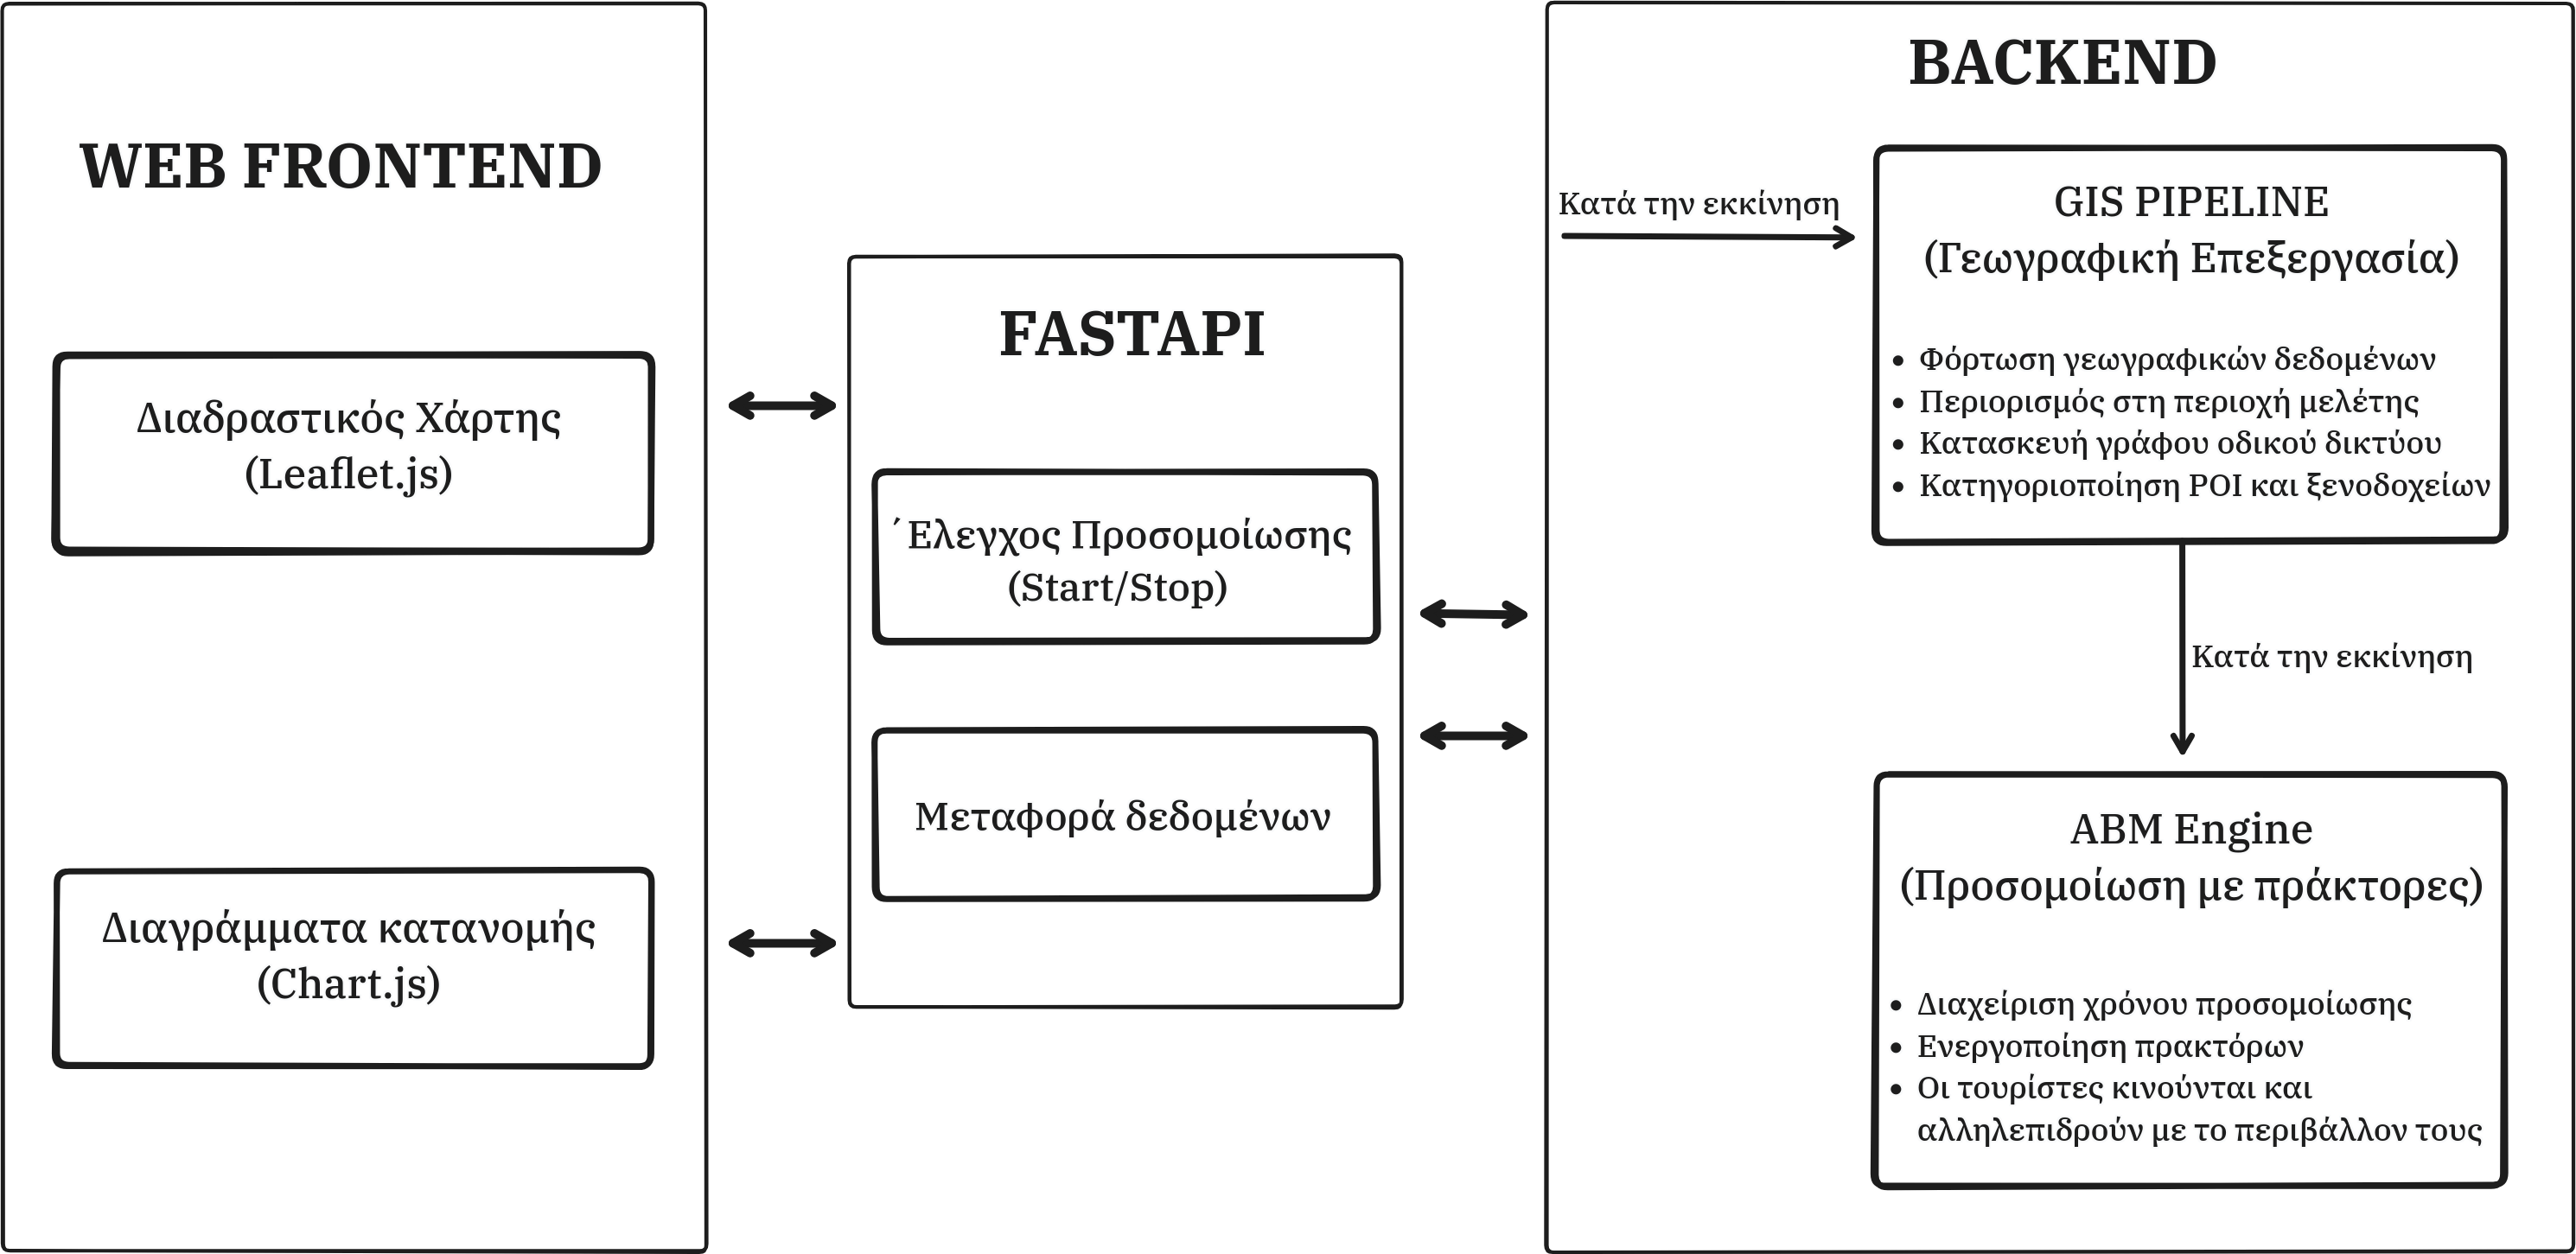
\includegraphics[width=\textwidth]{static/figures/system_architecture.png}
\caption{Αρχιτεκτονική Συστήματος}\label{system_architecture}
\end{figure}

\section{Σχεδιασμός Οδικού Δικτύου ως Γράφος}

Το οδικό δίκτυο αποτελεί τον χώρο κίνησης των πρακτόρων. Η
βασική σχεδιαστική απόφαση είναι η αναπαράστασή του ως μη
κατευθυνόμενος γράφος, όπου κάθε κόμβος αντιστοιχεί σε σημείο
διασταύρωσης ή άκρο δρόμου, και κάθε ακμή αντιστοιχεί σε τμήμα
δρόμου με γνωστή γεωμετρία. Αυτή η αναπαράσταση, όπως αναλύθηκε
στην Ενότητα 2.4, επιτρέπει την εφαρμογή αλγορίθμων πλοήγησης
και την ακριβή παρεμβολή θέσης πάνω στις ακμές.

Από το σύνολο των οδών που περιέχουν τα δεδομένα \en{OSM},
επιλέγονται μόνο εκείνες που επιτρέπουν πεζή κυκλοφορία,
αποκλείοντας ταχείες οδούς και αυτοκινητόδρομους που δεν είναι
προσβάσιμοι στους πεζούς. Η επιλογή αυτή εξασφαλίζει ότι η
κίνηση των πρακτόρων αντικατοπτρίζει ρεαλιστικά τη συμπεριφορά
των πεζών σε αστικό περιβάλλον.

Κάθε ακμή του γράφου αποκτά ένα βαθμολόγιο ελκυστικότητας που
συνδυάζει δύο παράγοντες: τον τύπο του δρόμου και την παρουσία
\en{POI} στην άμεση γειτονιά του. Αυτό το βαθμολόγιο
αντικατοπτρίζει την τάση των τουριστών να προτιμούν δρόμους με
εμπορική ή πολιτιστική δραστηριότητα, και αξιοποιείται από τον
αλγόριθμο πλοήγησης που περιγράφεται στην Ενότητα 4.4.2.

\section{Σχεδιασμός Πρακτόρων}

Το σύστημα περιλαμβάνει δύο διακριτούς τύπους πρακτόρων με
διαφορετική συμπεριφορά και ρόλο στην προσομοίωση. Και οι δύο
τύποι ζουν στον κοινό χώρο του μοντέλου, αλλά ο βαθμός
πολυπλοκότητάς τους διαφέρει σημαντικά.

\subsection{Μόνιμος Κάτοικος}

Ο μόνιμος κάτοικος \en{(resident)} αντιπροσωπεύει τον μόνιμο
πληθυσμό της πόλης. Είναι στατικός πράκτορας, δηλαδή δεν
κινείται κατά τη διάρκεια της προσομοίωσης, και ο ρόλος του
είναι να αποτυπώνει τον αντίκτυπο του τουρισμού στην ποιότητα
ζωής των κατοίκων μέσω μεταβλητής ευτυχίας.

Η ευτυχία \en{(happiness)} μεταβάλλεται ανάλογα με τον αριθμό
τουριστών που βρίσκονται στην άμεση γειτονιά του κατοίκου:
αυξάνεται όταν δεν υπάρχουν τουρίστες κοντά, μειώνεται
σταδιακά με την αύξηση του συνωστισμού και επαναφέρεται στην
αρχική τιμή στην αρχή κάθε νέας ημέρας. Η απλότητα αυτού του
μοντέλου είναι συνειδητή. Ο κάτοικος λειτουργεί ως
$``$αισθητήρας$"$ τουριστικής πίεσης στον χώρο, όχι ως
αυτόνομος πράκτορας με δικές του πρωτοβουλίες.

\subsection{Τουρίστας}

Ο τουρίστας \en{(tourist)} είναι ο πολυπλοκότερος πράκτορας
του συστήματος. Κινείται πάνω στο οδικό δίκτυο και εμφανίζει
σύνθετη ημερήσια συμπεριφορά που περιλαμβάνει φάσεις ύπνου,
ενεργή περιήγηση και επίσκεψη \en{POI}. Κάθε τουρίστας φέρει
χαρακτηριστικά περιβαλλοντικής επίδρασης (θόρυβος, ρύπανση)
και παρακολουθεί την ικανοποίησή του ανάλογα με τις συνθήκες
συνωστισμού που συναντά.

Ο τουρίστας όταν ανακαλύπτει ένα νέο σημείο ενδιαφέροντος,
κατευθύνεται προς αυτό και το επισκέπτεται. Διαθέτει ωστόσο
δυνατότητα παρεκτροπής. Για παράδειγμα, μπορεί να κάνει στάση
για καφέ καθώς κατευθύνεται προς ένα μουσείο. Σε αυτή την
περίπτωση, το καφέ γίνεται πρωτεύον στόχος του τουρίστα, ενώ
το μουσείο από πρωτεύον γίνεται δευτερεύον στόχος. Η απόφαση
παρεκτροπής είναι στοχαστική και εξαρτάται από το \en{tier}
του \en{POI}. Κανένας τουρίστας δεν επισκέπτεται δύο φορές
το ίδιο \en{POI}.

Η πλοήγηση στο οδικό δίκτυο βασίζεται σε υβριδικό αλγόριθμο
που συνδυάζει δύο κριτήρια: την ευθυγράμμιση με την κατεύθυνση
προς τον στόχο και την ελκυστικότητα της ακμής. Η στάθμιση
μεταξύ των δύο κριτηρίων προσαρμόζεται δυναμικά ανάλογα με
την απόσταση από τον στόχο, ώστε ο τουρίστας να διατηρεί
την κατεύθυνσή του όταν ο στόχος είναι μακριά, ενώ να
εξερευνά πιο ελεύθερα όταν βρίσκεται κοντά.

\subsection{Σύστημα Ιεραρχίας \en{POI}}

Τα Σημεία Ενδιαφέροντος κατηγοριοποιούνται σε τρία επίπεδα
βάσει της τουριστικής τους σημασίας και του τύπου εμπειρίας
που προσφέρουν. Η ιεράρχηση αυτή αντικατοπτρίζει την πραγματική
συμπεριφορά των τουριστών, οι οποίοι οργανώνουν την ημέρα τους
γύρω από λίγα κεντρικά αξιοθέατα και συμπληρώνουν την εμπειρία
τους με επισκέψεις σε εστιατόρια και καταστήματα.

Το \en{Tier A} περιλαμβάνει τα σημεία υψηλής τουριστικής αξίας,
όπως μουσεία, αξιοθέατα, μνημεία, αρχαιολογικούς χώρους και
παρόμοιους προορισμούς. Αποτελεί τον κύριο λόγο επίσκεψης μιας
πόλης. Το \en{Tier B} περιλαμβάνει καταστήματα εστίασης και
αναψυχής, που λειτουργούν ως δευτερεύοντες προορισμοί που
εμπλουτίζουν την εμπειρία της περιήγησης. Το \en{Tier C}
περιλαμβάνει καταστήματα λιανικής, που αποτελούν τριτεύοντες
προορισμούς ευκαιριακής επίσκεψης.

Ο αλγόριθμος επιλογής στόχου ακολουθεί αυστηρή ιεραρχία:
ο τουρίστας αναζητά πάντα πρώτα \en{POI Tier A}, και μόνο αν
δεν εντοπίσει κανένα στρέφεται σε κατώτερα \en{tiers}. Αυτή
η ιεραρχία εφαρμόζεται τόσο κατά την έναρξη της ημέρας όσο
και κατά την ελεύθερη περιπλάνηση. Η διάρκεια επίσκεψης
διαφέρει ανά \en{tier}, αντικατοπτρίζοντας τον διαφορετικό
χαρακτήρα κάθε κατηγορίας \en{POI}.

\section{Ξενοδοχεία και Ανάθεση Πρακτόρων}

Τα ξενοδοχεία αποτελούν τη βάση επιστροφής των τουριστών κατά
τις ώρες ύπνου και αντλούνται αυτόματα από τα δεδομένα \en{OSM}.
Σε περίπτωση που η βάση δεδομένων δεν περιέχει επαρκή αριθμό
ξενοδοχείων για την επιλεγμένη πόλη, το σύστημα χρησιμοποιεί
εναλλακτικά \en{POI} υψηλής επισκεψιμότητας ως σημεία αναφοράς,
εξασφαλίζοντας τη λειτουργία του μοντέλου ανεξαρτήτως της
πληρότητας των δεδομένων.

Κατά τη δημιουργία κάθε τουρίστα, το σύστημα του αναθέτει
αυτόματα ένα ξενοδοχείο μέσω αλγορίθμου ισορροπημένης κατανομής,
ο οποίος αποφεύγει την υπερφόρτωση συγκεκριμένων ξενοδοχείων.
Η ανάθεση παραμένει σταθερή για όλη τη διάρκεια της προσομοίωσης.

Η μετάβαση στη φάση ύπνου αντιμετωπίζεται με απλοποίηση.
Ο τουρίστας μεταφέρεται άμεσα στη θέση του ξενοδοχείου του,
αντί να πλοηγηθεί εκεί μέσω του οδικού δικτύου. Αυτή η
σχεδιαστική επιλογή είναι συνειδητή. Αποφεύγει πολυπλοκότητα
που δεν προσθέτει ερευνητική αξία, εφόσον το ενδιαφέρον της
προσομοίωσης εστιάζεται στη δραστηριότητα κατά τις ώρες εγρήγορσης.
	\chapter{Υλοποίηση}

Στο παρόν κεφάλαιο παρουσιάζεται η υλοποίηση του συστήματος,
όπως αυτή προέκυψε από τις σχεδιαστικές αποφάσεις του
Κεφαλαίου 4. Αρχικά παρουσιάζονται τα εργαλεία και οι
τεχνολογίες που επιλέχθηκαν, και στη συνέχεια αναλύονται
διαδοχικά τα τέσσερα βασικά στρώματα του συστήματος:
το \en{pipeline} επεξεργασίας γεωγραφικών δεδομένων,
η υλοποίηση των πρακτόρων, το \en{REST API} και το
\en{web frontend}.

\section{Εργαλεία και Τεχνολογίες}

Η υλοποίηση του συστήματος βασίζεται αποκλειστικά σε ανοιχτού
κώδικα εργαλεία και βιβλιοθήκες. Στο επίπεδο του \en{backend},
η γλώσσα προγραμματισμού \en{Python} αποτέλεσε την κύρια
επιλογή λόγω του πλούσιου οικοσυστήματος βιβλιοθηκών για
επιστημονικό υπολογισμό, γεωγραφικά δεδομένα και
μοντελοποίηση πρακτόρων.

Για την υλοποίηση του \en{ABM} χρησιμοποιήθηκε το
\en{framework Mesa}, το οποίο παρέχει τις βασικές αφαιρέσεις
για πράκτορες, μοντέλα και χώρους, όπως αναλύθηκε στην
Ενότητα 2.2. Ο χώρος κίνησης των πρακτόρων υλοποιείται μέσω
του \en{ContinuousSpace} του \en{Mesa}, που επιτρέπει
τοποθέτηση και μετακίνηση σε συνεχή δισδιάστατο χώρο με
μετρικές αποστάσεις.

Για την επεξεργασία γεωγραφικών δεδομένων χρησιμοποιήθηκαν
οι βιβλιοθήκες \en{GeoPandas} και \en{Shapely}, ενώ για τη
μετατροπή συντεταγμένων μεταξύ γεωγραφικών συστημάτων αναφοράς
η βιβλιοθήκη \en{PyProj}. Η κατασκευή και διαχείριση του γράφου
οδικού δικτύου υλοποιήθηκε με τη βιβλιοθήκη \en{NetworkX}, όπως
αναλύθηκε στην Ενότητα 2.4.3. Το \en{REST API} εκθέτεται μέσω
του \en{framework FastAPI}, το οποίο επιλέχθηκε για την υψηλή
του απόδοση και τη διαισθητική δήλωση \en{endpoints}.

Στο επίπεδο του \en{frontend}, η οπτικοποίηση του χάρτη
υλοποιείται με τη βιβλιοθήκη \en{Leaflet.js}, που παρέχει
διαδραστικό χάρτη βασισμένο σε \en{tiles} του
\en{OpenStreetMap}. Τα γραφήματα κατανομών υλοποιούνται με
τη βιβλιοθήκη \en{Chart.js}. Και οι δύο βιβλιοθήκες
εκτελούνται αποκλειστικά στον \en{browser}, χωρίς εξαρτήσεις
από εξωτερικά \en{frameworks}.

\section{\en{Pipeline} Φόρτωσης \en{GIS} Δεδομένων}

Το σύνολο της προεπεξεργασίας γεωγραφικών δεδομένων υλοποιείται
στη συνάρτηση \en{load\_gis\_model()} του αρχείου \en{main.py}.
Η συνάρτηση αυτή εκτελείται μία φορά κατά την εκκίνηση της
εφαρμογής και επιστρέφει όλα τα απαραίτητα δεδομένα για τη
δημιουργία του μοντέλου: τον γράφο οδικού δικτύου, τις
γεωμετρίες ακμών, τα \en{POI} και τα ξενοδοχεία.

Η συνάρτηση δέχεται ως παράμετρο το όνομα της πόλης
\en{(city\_name)}, το οποίο από προεπιλογή ορίζεται σε
$``$Πάτρα$"$. Η πόλη αναζητείται στο
\en{layer\ gis\_osm\_places\_free\_1} του αρχείου \en{Shapefile},
και σε περίπτωση πολλαπλών αποτελεσμάτων με το ίδιο όνομα
επιλέγεται αυτόματα η μεγαλύτερη σε πληθυσμό ή σημαντικότερη
κατηγορίας \en{(city $>$ town $>$ village)}. Γύρω από το κεντρικό
σημείο της πόλης δημιουργείται ζώνη αναφοράς \en{(buffer)}
ακτίνας 1.000 μέτρων στο σύστημα \en{EPSG:2100}, η οποία
μετατρέπεται σε ορθογώνιο πλαίσιο \en{(bounding box)} στο σύστημα
\en{WGS84}. Το πλαίσιο αυτό χρησιμοποιείται ως φίλτρο κατά τη
φόρτωση όλων των υπόλοιπων \en{layers} (οδοί, \en{POI}),
περιορίζοντας την ανάλυση αποκλειστικά στην περιοχή μελέτης και
μειώνοντας σημαντικά τον χρόνο επεξεργασίας.

\subsection{Φιλτράρισμα Οδών}

Από το \en{layer gis\_osm\_roads\_free\_1} φορτώνονται μόνο οι
οδοί εντός του \en{bounding box} της επιλεγμένης πόλης. Στη
συνέχεια εφαρμόζεται φίλτρο βάσει του πεδίου \en{fclass}, το
οποίο περιγράφει τον τύπο κάθε οδού. Διατηρούνται αποκλειστικά
οι κατηγορίες που επιτρέπουν πεζή κυκλοφορία: \en{footway, path,
pedestrian, steps, residential, living\_street, service,
unclassified, tertiary, secondary} και \en{primary}. Οδοί ταχείας
κυκλοφορίας \en{(motorway, trunk)} και σιδηροδρομικές γραμμές
αποκλείονται πλήρως.

Μετά το φιλτράρισμα, οι γεωμετρίες μετατρέπονται στο σύστημα
συντεταγμένων \en{EPSG:2100} (ΕΓΣΑ '87), το οποίο διατηρεί
αποστάσεις σε μέτρα. Αυτή η μετατροπή είναι απαραίτητη για τον
ακριβή υπολογισμό αποστάσεων και ταχυτήτων κατά την κίνηση των
πρακτόρων. Εάν ο αριθμός των φιλτραρισμένων οδών υπερβαίνει το
όριο των 5.000 τμημάτων, το σύστημα ζητά επιβεβαίωση από τον
χρήστη, καθώς η κατασκευή του γράφου για τόσο μεγάλο δίκτυο
απαιτεί σημαντικό υπολογιστικό χρόνο.

\subsection{Κατασκευή Γράφου}

Η κατασκευή του γράφου από τα ακατέργαστα τμήματα οδών είναι το
υπολογιστικά εντατικότερο βήμα του \en{pipeline} και υλοποιείται
σε τρεις φάσεις.

Στην πρώτη φάση εντοπίζονται τα σημεία τομής μεταξύ τμημάτων οδών.
Για κάθε ζεύγος τμημάτων ελέγχεται αν τέμνονται γεωμετρικά. Τα
άκρα όλων των τμημάτων (αρχή και τέλος κάθε \en{LineString})
προστίθενται αυτόματα ως υποψήφια σημεία κόμβων. Τα σημεία τομής
που δεν συμπίπτουν με άκρο (εσωτερικές τομές) εντοπίζονται και
καταγράφονται κι αυτά ως υποψήφια σημεία κόμβων.

Στη δεύτερη φάση δημιουργούνται οι κόμβοι του γράφου. Κάθε
μοναδικό σημείο τομής μετατρέπεται σε κόμβο με μοναδικό
αναγνωριστικό. Για την αντιμετώπιση της γεωμετρικής ανακρίβειας
των δεδομένων \en{OSM}, εφαρμόζεται τεχνική \en{snapping}, όπου
συντεταγμένες που απέχουν λιγότερο από 5 μέτρα στρογγυλοποιούνται
στο πλησιέστερο πολλαπλάσιο του 5, ώστε να αντιστοιχιστούν στον
ίδιο κόμβο. Χωρίς αυτή την τεχνική, μικρές αριθμητικές αποκλίσεις
στα δεδομένα θα δημιουργούσαν χιλιάδες διπλότυπους κόμβους και
αποσυνδεδεμένα τμήματα δικτύου.

Στην τρίτη φάση κάθε τμήμα οδού διασπάται στα σημεία που
εντοπίστηκαν κοντά του (εντός \en{snap tolerance}). Για κάθε τμήμα
υπολογίζεται η προβολή κάθε κόμβου πάνω στη γραμμή, και το τμήμα
διασπάται σε υποτμήματα μεταξύ διαδοχικών προβολών. Κάθε υποτμήμα
αποθηκεύεται ως ακμή του γράφου με τη γεωμετρία του
\en{(LineString)} και αντίστοιχη αντίστροφη γεωμετρία για την
κίνηση προς αμφότερες τις κατευθύνσεις.

\begin{figure}[H] \centering
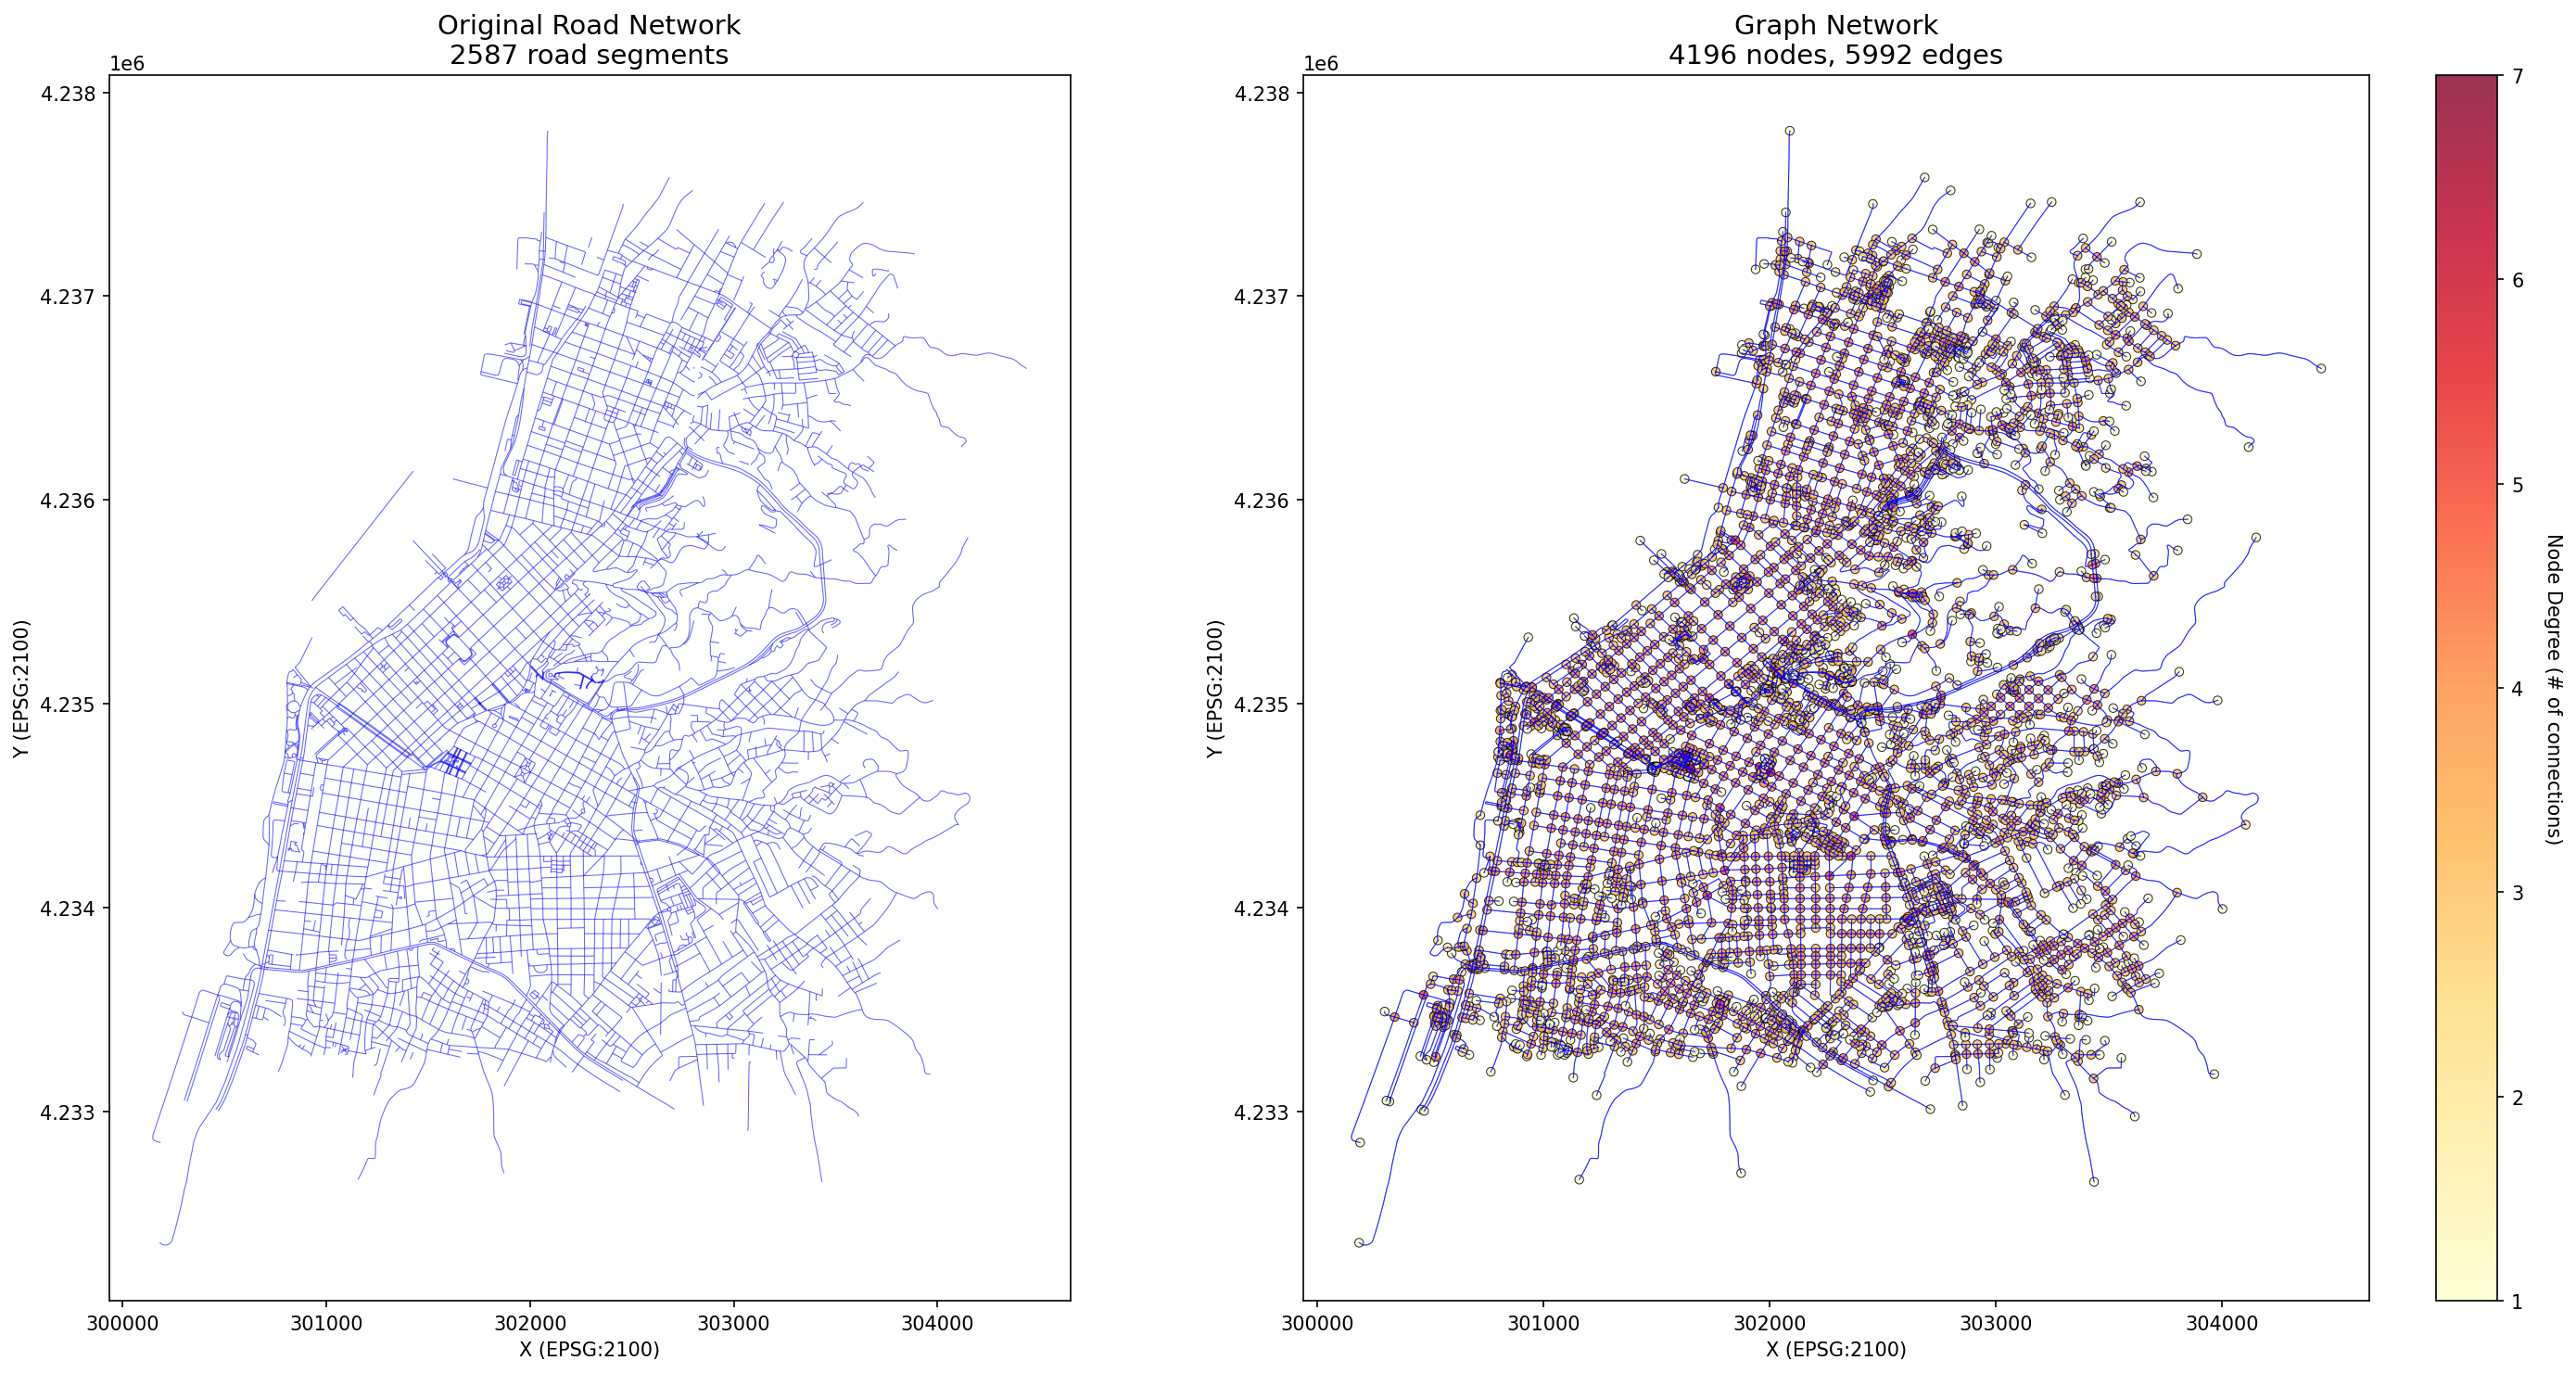
\includegraphics[width=\textwidth]{static/figures/road_network_graph.png}
\caption{Κατασκευή Γράφου Οδικού Δικτύου}\label{road_network_graph}
\end{figure}

\subsection{Ελκυστικότητα Δρόμων}

Μετά την κατασκευή του γράφου, κάθε ακμή αποκτά βαθμολογία
ελκυστικότητας \en{(attractiveness score)} που χρησιμοποιείται
από τον αλγόριθμο πλοήγησης των τουριστών. Η βαθμολογία
υπολογίζεται ως άθροισμα δύο συνιστωσών.

Η πρώτη συνιστώσα είναι η βασική βαθμολογία τύπου οδού
\en{(base score)}, όπου: \en{pedestrian=5, footway=4,
living\_street=3, residential=2, tertiary/secondary/primary=1.}
Οι πεζόδρομοι λαμβάνουν υψηλότερη βαθμολογία γιατί είναι φυσικά
πιο ελκυστικοί για τους πεζούς τουρίστες.

Η δεύτερη συνιστώσα είναι η βαθμολογία \en{POI (poi score)}, όπου
για κάθε ακμή δημιουργείται \en{buffer} 30 μέτρων και
καταμετρούνται τα \en{POI} που περιέχονται σε αυτή. Κάθε
\en{POI Tier A} συνεισφέρει 10 μονάδες, κάθε \en{Tier B} 3 μονάδες
και κάθε \en{Tier C} 1 μονάδα. Η τελική βαθμολογία είναι το
άθροισμα \en{base score} και \en{poi score}, και αποθηκεύεται ως
χαρακτηριστικό της ακμής στον γράφο.

\subsection{Φόρτωση \en{POI} και Ξενοδοχείων}

Τα σημεία ενδιαφέροντος φορτώνονται από το
\en{layer gis\_osm\_pois\_free\_1} εντός του \en{bounding box}
της πόλης. Για κάθε \en{POI} εξετάζεται το πεδίο \en{fclass} και
κατατάσσεται στο αντίστοιχο \en{tier}:
\begin{itemize}
\item \en{Tier A} για μουσεία, αξιοθέατα, μνημεία, αρχαιολογικούς
χώρους, κάστρα, πάρκα θεματικής αναψυχής και εμπορικά κέντρα
\item \en{Tier B} για καφετέριες, εστιατόρια, \en{fast food, bar}
και \en{pub}
\item \en{Tier C} για καταστήματα ρουχισμού, βιβλιοπωλεία,
αρτοποιεία, σούπερ μάρκετ και δώρα.
\end{itemize}
\en{POI} που δεν ανήκουν σε κανέναν από τους παραπάνω τύπους
αγνοούνται. Κάθε \en{POI} αποθηκεύεται ως λεξικό με μοναδικό
αναγνωριστικό, όνομα, γεωμετρία, τύπο \en{fclass} και \en{tier}.

Τα ξενοδοχεία αναζητούνται στο ίδιο \en{layer} με τύπους
\en{hotel, hostel, motel} και \en{guest\_house}. Εάν εντοπιστούν
λιγότερα από 3, το σύστημα επεκτείνει αναζήτηση σε \en{POI} τύπου
\en{accommodation} και στη συνέχεια, αν χρειαστεί, χρησιμοποιεί
τα πρώτα διαθέσιμα \en{POI} υψηλής επισκεψιμότητας (εστιατόρια,
καφετέριες, αξιοθέατα) ως υποκατάστατα. Αυτή η λογική εναλλακτικής
αναζήτησης εξασφαλίζει τη λειτουργία του μοντέλου ακόμα και για
πόλεις με ελλιπή καταγραφή ξενοδοχείων στα δεδομένα \en{OSM}.

\section{Υλοποίηση Πρακτόρων}

Οι πράκτορες υλοποιούνται στο αρχείο \en{agents.py}. Η κλάση
\en{ResidentAgent} κληρονομεί από την \en{Agent} του \en{Mesa}
και υλοποιεί απλή λογική ενημέρωσης ευτυχίας. Η κλάση
\en{TouristAgent} κληρονομεί επίσης από \en{Agent} και υλοποιεί
το σύνολο της σύνθετης συμπεριφοράς που περιγράφηκε στην
Ενότητα 4.4.2. Και οι δύο κλάσεις ενσωματώνονται στην κλάση
\en{CityModel}, η οποία κληρονομεί από \en{Model} του \en{Mesa}
και διαχειρίζεται τον χρόνο, τον χώρο και την ενεργοποίηση των
πρακτόρων.

\subsection{Ημερήσιος Κύκλος Τουρίστα}

Ο ημερήσιος κύκλος του τουρίστα υλοποιείται στη μέθοδο \en{step()}
της \en{TouristAgent}, η οποία καλείται σε κάθε βήμα προσομοίωσης
(10 λεπτά). Η λογική βασίζεται στον τρέχοντα χρόνο της
προσομοίωσης \en{(current\_hour, current\_min)} και στην εσωτερική
μεταβλητή κατάστασης \en{state}.

Κατά τις ώρες 00:00–08:00, εάν ο τουρίστας δεν βρίσκεται ήδη σε
κατάσταση \en{sleeping}, μεταφέρεται στο ξενοδοχείο του (μέθοδος
\en{teleport\_to\_hotel()}) και η κατάστασή του ορίζεται σε
\en{sleeping}. Η ικανοποίησή του επαναφέρεται στην αρχική τιμή
0.7. Στις 8:00 π.μ., εάν η κατάσταση είναι \en{sleeping}, καλείται
η μέθοδος \en{\_initialize\_daily\_targets()} που σαρώνει ακτίνα
100 μέτρων για \en{POI} και ορίζει τον πρώτο στόχο της ημέρας.

Κατά τις ενεργές ώρες, ο τουρίστας βρίσκεται σε μία από τις εξής
καταστάσεις: \en{walking\_to\_tier\_a, walking\_to\_tier\_b,
walking\_to\_tier\_c} (μετάβαση προς \en{POI}),
\en{visiting\_tier\_a, visiting\_tier\_b, visiting\_tier\_c}
(παραμονή σε \en{POI}), ή \en{casual\_wandering} (ελεύθερη
περιπλάνηση χωρίς στόχο). Η διάρκεια επίσκεψης ορίζεται ως
180 λεπτά για \en{Tier A}, 60 λεπτά για \en{Tier B} και
20 λεπτά για \en{Tier C}. Τα \en{POI Tier A} δέχονται επισκέπτες
μέχρι τις 18:00 και κλείνουν στις 20:00. Κατά τα μεσάνυχτα,
η μέθοδος \en{\_reset\_daily\_attributes()} του \en{CityModel}
επαναφέρει την ευτυχία κατοίκων, την ικανοποίηση τουριστών και
τις πιθανότητες παρεκτροπής σε αρχικές τιμές.

\begin{figure}[H] \centering
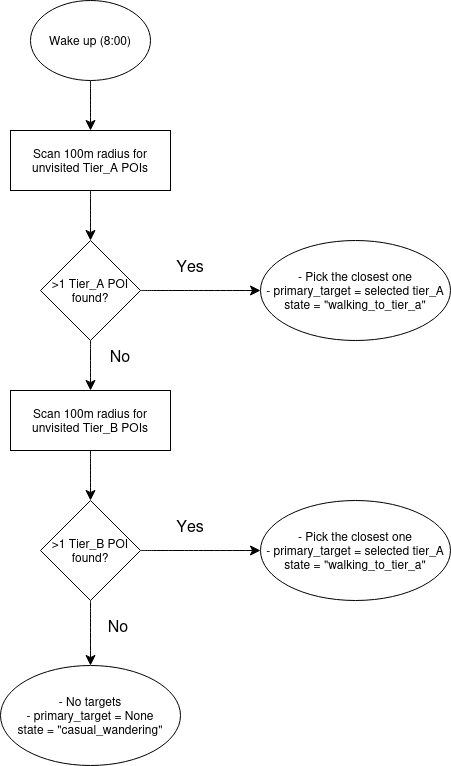
\includegraphics[width=0.5\textwidth]{static/figures/wake_up.png}
\caption{Επιλογή Στόχου κατά το Ξύπνημα}\label{wake_up}
\end{figure}

\subsection{\en{Forward Vision Scan} και \en{Detour} Λογική}

Ο μηχανισμός \en{forward vision scan} υλοποιείται στη μέθοδο 
\en{\_forward\_vision\_scan()}, η οποία καλείται σε κάθε βήμα
όταν ο τουρίστας βρίσκεται σε κατάσταση μετάβασης προς
\en{POI}. Η μέθοδος αναζητάει ανεπίσκεπτα \en{POI Tier B} ή \en{C}
που βρίσκονται εντός ακτίνας 30 μέτρων από την τρέχουσα θέση του
τουρίστα.

Για λόγους απόδοσης, κατά την εκκίνηση του μοντέλου κατασκευάζεται
μία δομή \en{KDTree (scipy.spatial.KDTree)} πάνω στις συντεταγμένες
όλων των \en{POI}. Αντί να επαναλαμβάνεται πλήρης σάρωση όλων των
\en{POI} σε κάθε βήμα και για κάθε τουρίστα, το \en{KDTree}
επιτρέπει ανάκτηση μόνο των \en{POI} εντός της επιθυμητής ακτίνας
σε \en{O(log n)} χρόνο, μειώνοντας σημαντικά το υπολογιστικό κόστος
κατά την εκτέλεση της προσομοίωσης.

Έπειτα, για κάθε \en{POI} εντός ακτίνας υπολογίζεται η γωνία μεταξύ
της κατεύθυνσης προς τον τρέχοντα στόχο και της κατεύθυνσης προς το
\en{POI}, μέσω εσωτερικού γινομένου \en{(dot product)} των
αντίστοιχων μοναδιαίων διανυσμάτων. Εάν η γωνία είναι μικρότερη
από 30 μοίρες, το \en{POI} βρίσκεται εντός του οπτικού κώνου και
καλείται η μέθοδος \en{\_consider\_poi\_detour()}.

Η μέθοδος \en{\_consider\_poi\_detour()} αποφασίζει στοχαστικά αν
θα γίνει παρεκτροπή, η οποία συμβαίνει με πιθανότητα 30\% για
\en{POI Tier B} και 20\% για \en{Tier C}. Σε περίπτωση
παρεκτροπής, ο τρέχων πρωτεύων στόχος αποθηκεύεται ως δευτερεύων
\en{(secondary\_target)} και το \en{POI} ορίζεται ως νέος
πρωτεύων στόχος. Μετά την ολοκλήρωση της επίσκεψης, η μέθοδος
\en{\_exit\_poi()} ελέγχει αν ο δευτερεύων στόχος βρίσκεται εντός
300 μέτρων. Aν ναι, αποκαθίσταται ως πρωτεύων στόχος, αλλιώς ο
τουρίστας περνά σε κατάσταση \en{casual\_wandering}. Μετά από
κάθε επίσκεψη, η αντίστοιχη πιθανότητα παρεκτροπής μειώνεται
κατά 0.15 για \en{Tier B} (ελάχιστο 0.15) και 0.05 για
\en{Tier C} (ελάχιστο 0.05).

\begin{figure}[H] \centering
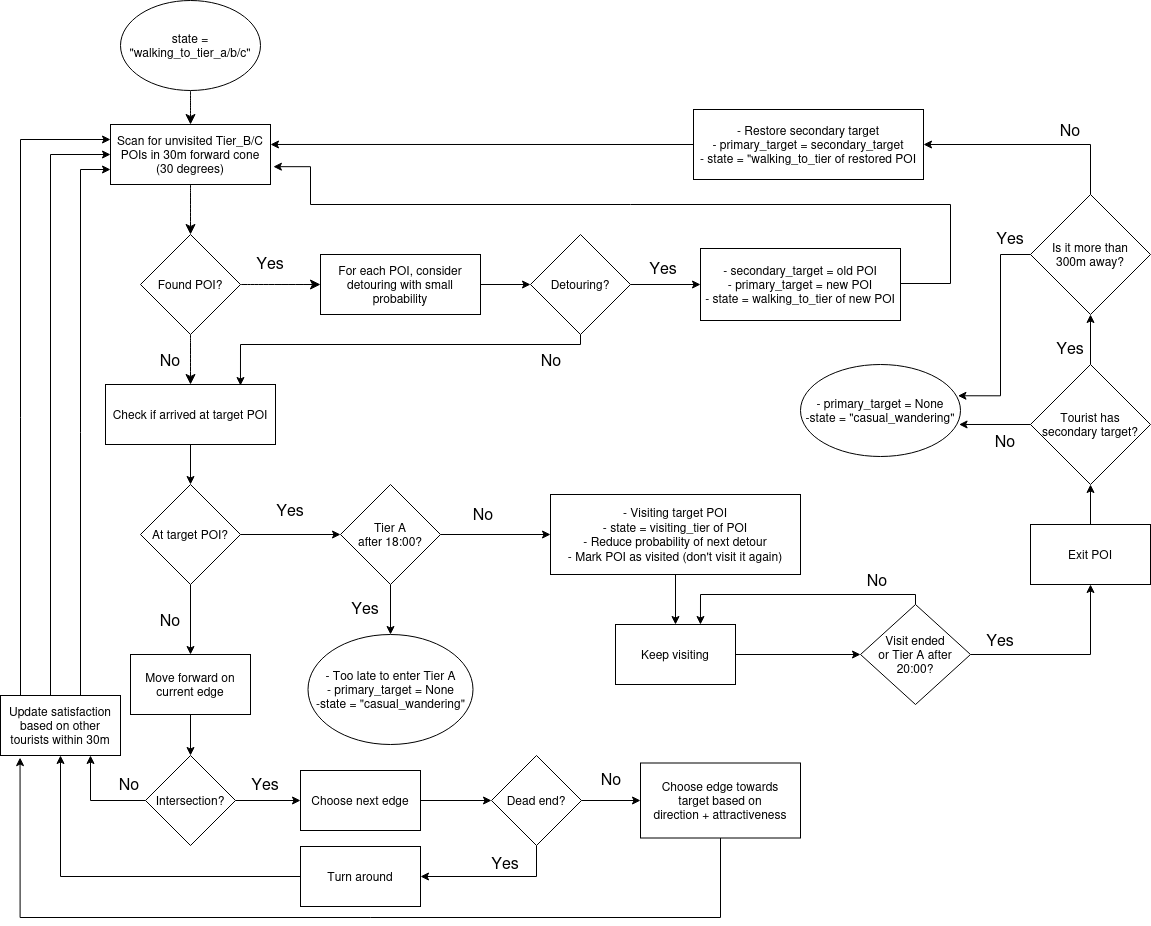
\includegraphics[width=\textwidth]{static/figures/walking_to_tier.png}
\caption{Βασικό Διάγραμμα Ροής}\label{walking_to_tier-100-23r}
\end{figure}

\begin{figure}[H] \centering
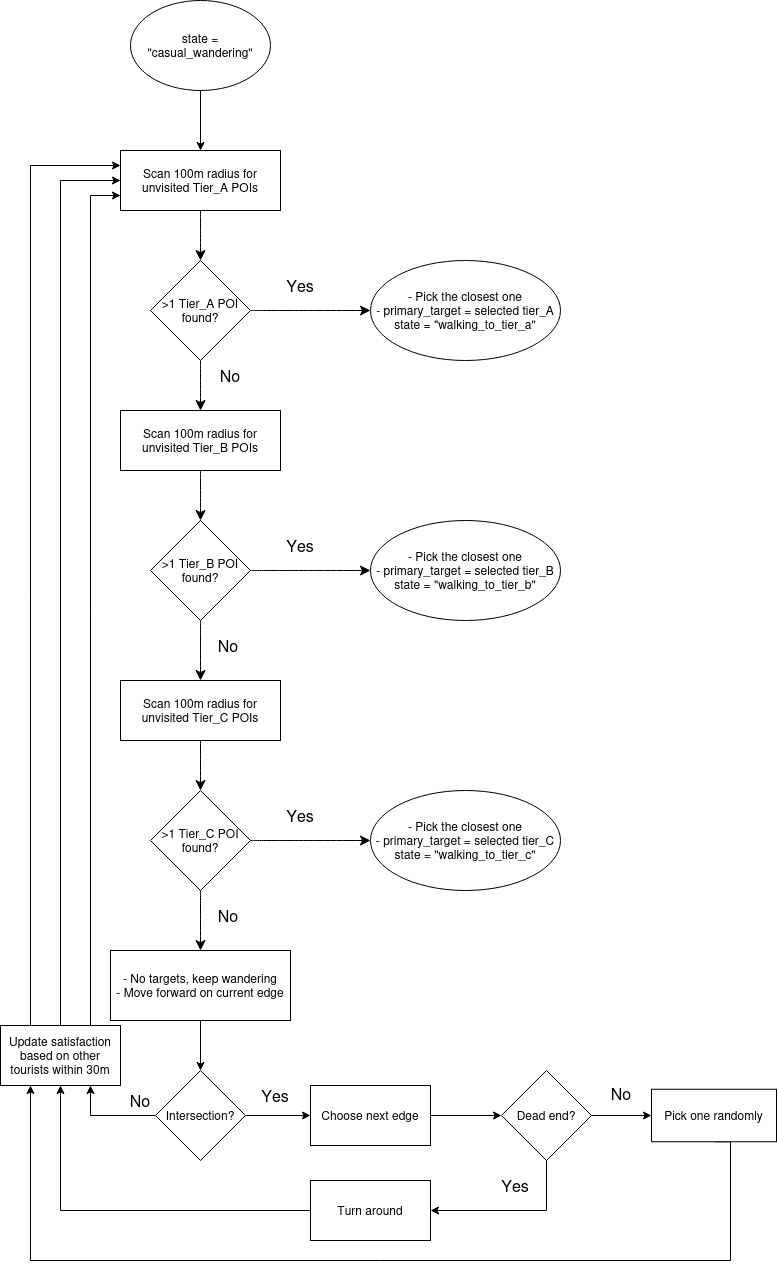
\includegraphics[width=0.8\textwidth]{static/figures/casual_wandering.png}
\caption{Περίπτωση Περιπλάνησης}\label{casual_wandering}
\end{figure}

\subsection {Υβριδική Εύρεση Διαδρομής}

Η κίνηση πάνω στο γράφο υλοποιείται στη μέθοδο
\en{\_move\_on\_graph()}. Σε κάθε βήμα, ο τουρίστας προχωρά κατά
\en{speed} μέτρα πάνω στην τρέχουσα ακμή
\en{(pos\_on\_edge += speed)}. Όταν η \en{pos\_on\_edge} υπερβεί
το μήκος της ακμής, ο τουρίστας έχει φτάσει στον επόμενο κόμβο και
καλείται η μέθοδος \en{\_choose\_next\_edge()}. Η τρέχουσα θέση
στον χώρο υπολογίζεται με γεωμετρική παρεμβολή πάνω στη
\en{LineString} της ακμής (μέθοδος \en{interpolate} της
\en{Shapely}) και μετατρέπεται σε συντεταγμένες μοντέλου.

Η επιλογή επόμενης ακμής υλοποιείται στη μέθοδο
\en{\_choose\_next\_edge()}. Εάν ο τουρίστας δεν έχει ενεργό
στόχο, επιλέγει τυχαία μεταξύ των διαθέσιμων γειτονικών κόμβων
(αποφεύγοντας άμεση επιστροφή). Εάν έχει στόχο, καλείται η
μέθοδος \en{\_choose\_edge\_toward\_target()}.

Στη μέθοδο \en{\_choose\_edge\_toward\_target()} κάθε γειτονικός
κόμβος βαθμολογείται ως εξής: υπολογίζεται η ευθυγράμμιση
\en{(alignment)} ως \en{dot product} μεταξύ του μοναδιαίου
διανύσματος προς τον στόχο και του μοναδιαίου διανύσματος προς τον
γείτονα, ενώ αρνητικές τιμές (οπισθοδρόμηση) μηδενίζονται.
Η τελική βαθμολογία υπολογίζεται ως: \en{score = alignment × 0.8 +
(attractiveness / 10) × 0.2} όταν ο στόχος απέχει άνω των
200 μέτρων (μακρινός στόχος), και \en{score = alignment ×
attractiveness} όταν είναι κοντά. Η επιλογή γίνεται πιθανοτικά
βάσει των κανονικοποιημένων βαθμολογιών, με πιθανότητα τυχαίας
εξερεύνησης 5\% για μακρινό στόχο και 15\% για κοντινό.

\subsection{Μετρικές Ευτυχίας και Ικανοποίησης}

Η ευτυχία των κατοίκων ενημερώνεται στη μέθοδο
\en{\_update\_happiness()} της \en{ResidentAgent}. Σε κάθε βήμα
κατά τις ώρες κινητικότητας (8:00–24:00), μετράται ο αριθμός τουριστών
εντός ακτίνας 30 μέτρων μέσω της μεθόδου \en{get\_neighbors()} του
\en{ContinuousSpace}. Οι κανόνες ενημέρωσης είναι: +0.02 εάν δεν
υπάρχουν τουρίστες, +0.005 για 1–3 τουρίστες, -0.01 για 4–10
τουρίστες, -0.03 για άνω των 10. Η τιμή περιορίζεται πάντα στο
διάστημα [0.0, 1.0].

Η ικανοποίηση των τουριστών ενημερώνεται με αντίστοιχο τρόπο στη
μέθοδο \en{\_update\_satisfaction()} της \en{TouristAgent} μετά από
κάθε βήμα κίνησης. Με τον ίδιο μηχανισμό \en{get\_neighbors()}
καταμετρούνται οι γειτονικοί τουρίστες εντός 30 μέτρων: η ικανοποίηση
αυξάνεται κατά +0.01 εάν υπάρχουν έως 5 τουρίστες, παραμένει
αμετάβλητη για 6–15, και μειώνεται κατά -0.02 για άνω των 15.
Και αυτή η τιμή περιορίζεται στο [0.0, 1.0].

Η παραγωγή των \en{heatmaps} υλοποιείται στη μέθοδο
\en{generate\_heatmap()} του \en{CityModel}. Ο χώρος διαιρείται σε
πλέγμα κελιών 10×10 μέτρων. Για κάθε ενεργό τουρίστα (εκτός κατάστασης
\en{sleeping}), προστίθεται η τιμή \en{noise} ή \en{pollution} στο
κελί που βρίσκεται, και το 30\% της τιμής στα 8 γειτονικά κελιά,
προσομοιώνοντας τη χωρική διάχυση του θορύβου και της ρύπανσης.

\section{\en{REST API}}

Το \en{REST API} υλοποιείται με \en{FastAPI} στο αρχείο \en{main.py}.
Κατά την εκκίνηση \en{(startup event)}, καλείται η
\en{load\_gis\_model()} και δημιουργείται το \en{CityModel}. Το
μοντέλο αποθηκεύεται σε καθολική μεταβλητή και είναι προσβάσιμο από
όλα τα \en{endpoints}. Τα αρχεία του \en{frontend} σερβίρονται ως
στατικά αρχεία από τον φάκελο \en{static/}.

Το \en{endpoint GET /state} επιστρέφει την πλήρη κατάσταση της
προσομοίωσης, δηλαδή τον τρέχοντα χρόνο, τη λίστα όλων των πρακτόρων
με θέση και χαρακτηριστικά, τη λίστα ξενοδοχείων και τη λίστα \en{POI}.
Οι συντεταγμένες μετατρέπονται από \en{EPSG}:2100 σε \en{WGS84}
(γεωγραφικό πλάτος/μήκος) μέσω του \en{Transformer} της \en{PyProj},
ώστε να είναι απευθείας χρησιμοποιήσιμες από το \en{Leaflet.js}.

Το \en{endpoint POST /step} εκτελεί ένα βήμα προσομοίωσης
\en{(model.step())} και επιστρέφει την ενημερωμένη κατάσταση των
πρακτόρων. Το \en{endpoint POST /skip\_to\_morning} καλεί τη μέθοδο
\en{skip\_to\_morning()} του μοντέλου, η οποία ορίζει τον χρόνο σε
08:00, τηλεμεταφέρει όλους τους τουρίστες στα ξενοδοχεία τους και
επαναφέρει τις μεταβλητές ευημερίας. Τα \en{endpoints
GET /heatmap/noise} και \en{GET /heatmap/pollution} καλούν τη
\en{generate\_heatmap()} και επιστρέφουν το πλέγμα τιμών μαζί με
τις γεωγραφικές συντεταγμένες κάθε κελιού σε \en{WGS84}. Τα
\en{endpoints GET /distribution/happiness} και
\en{GET /distribution/satisfaction} επιστρέφουν ιστόγραμμα κατανομής
των αντίστοιχων μεταβλητών σε 10 \en{bins} του διαστήματος [0, 1].

\section{\en{Frontend} Οπτικοποίηση}

Το \en{frontend} υλοποιείται σε δύο αρχεία: \en{index.html} που
ορίζει τη δομή της σελίδας και φορτώνει τις εξαρτήσεις, και
\en{map.js} που περιέχει όλη τη λογική οπτικοποίησης και
αλληλεπίδρασης. Κατά τη φόρτωση της σελίδας, καλείται το
\en{endpoint /state} και αρχικοποιείται ο χάρτης με τις θέσεις
πρακτόρων, \en{POI} και ξενοδοχείων.

\subsection{Χάρτης \en{Leaflet} και \en{Layers}}

Ο χάρτης αρχικοποιείται κεντραρισμένος στην Πάτρα με \en{zoom level}
13. Ως υπόβαθρο χρησιμοποιούνται \en{tiles} του \en{OpenStreetMap}.
Τα δεδομένα οργανώνονται σε πέντε ανεξάρτητα \en{LayerGroups:
Residents, Tourists, Hotels, POIs} και \en{Heatmap}. Ο χρήστης
μπορεί να ενεργοποιεί ή να απενεργοποιεί κάθε \en{layer} ανεξάρτητα
μέσω του ενσωματωμένου \en{layer control} του \en{Leaflet}.

Οι κάτοικοι απεικονίζονται ως μπλε κύκλοι και οι τουρίστες ως
κόκκινοι κύκλοι \en{(CircleMarker)}. Κάθε πράκτορας φέρει \en{popup}
με τα πλήρη χαρακτηριστικά του. Για τους κατοίκους εμφανίζεται η
τιμή ευτυχίας, ενώ για τους τουρίστες εμφανίζονται θόρυβος, ρύπανση,
ικανοποίηση, τρέχουσα κατάσταση, πρωτεύων και δευτερεύων στόχος.
Τα ξενοδοχεία απεικονίζονται με μπλε \en{marker} και τα \en{POI}
με έγχρωμους \en{markers} διαφορετικού μεγέθους ανά \en{tier}
(πράσινος/μεγάλος για \en{Tier A}, κίτρινος/μεσαίος για \en{Tier B},
πορτοκαλί/μικρός για \en{Tier C}).

\begin{figure}[H] \centering
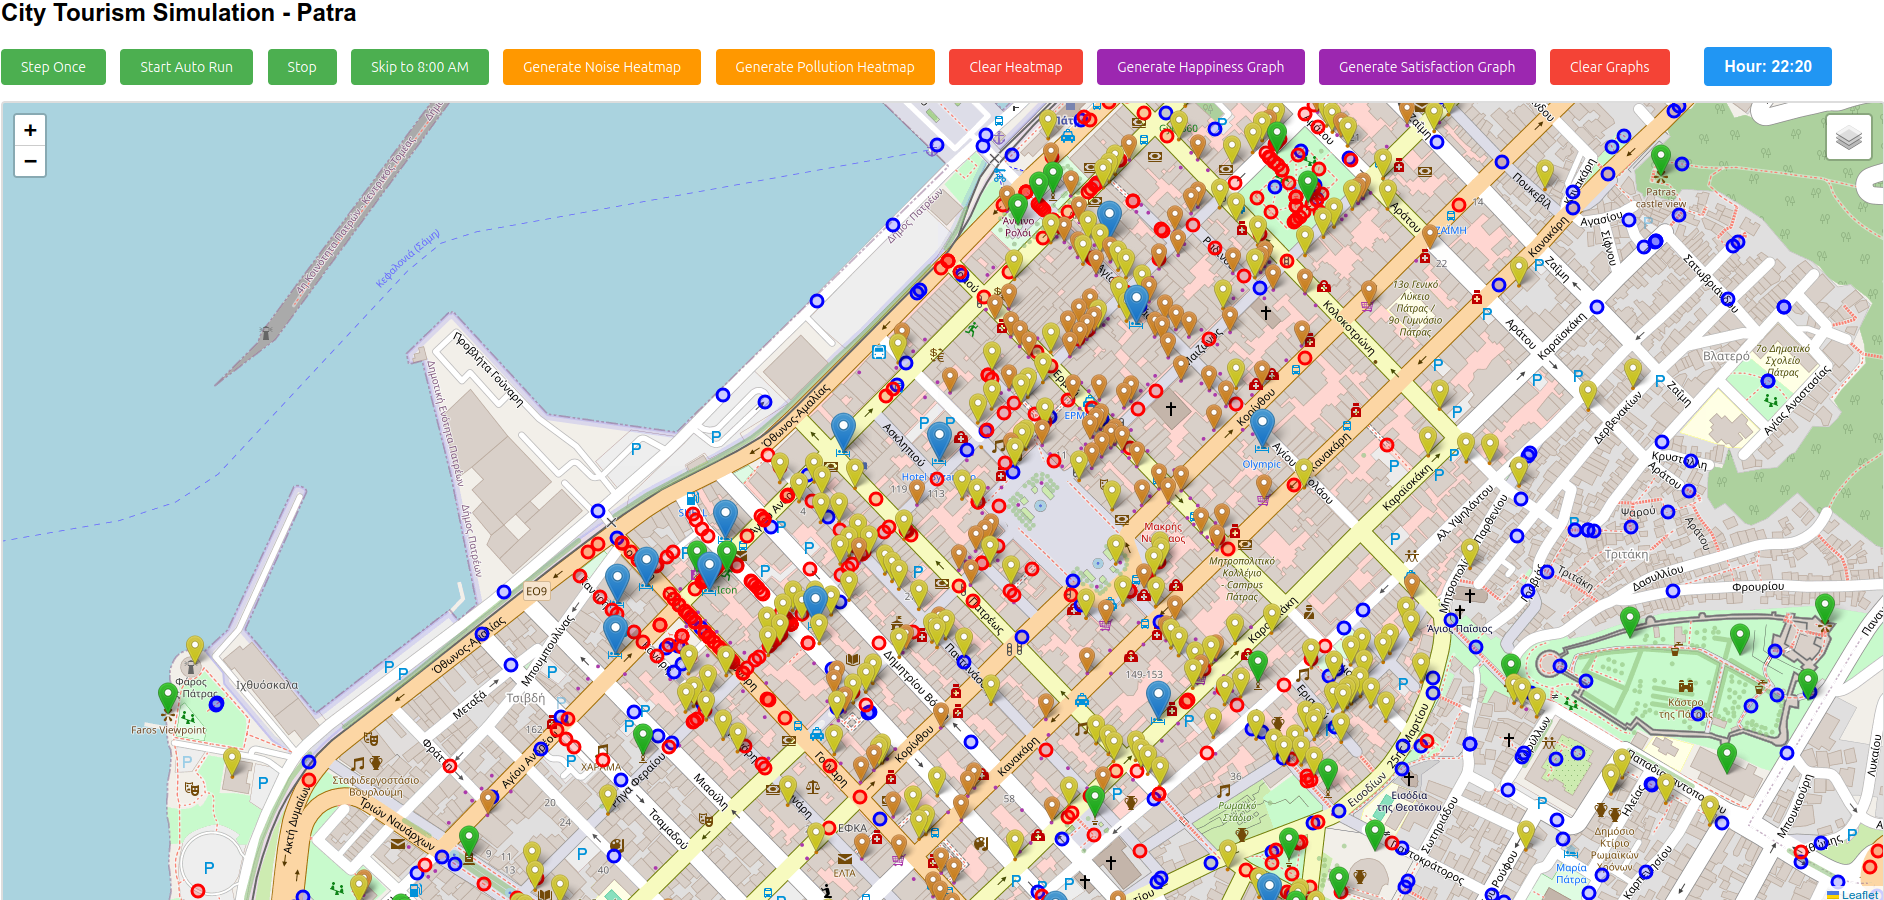
\includegraphics[width=\textwidth]{static/figures/map.png}
\caption{Χάρτης \en{Leaflet}}\label{map}
\end{figure}

\subsection{\en{Heatmaps} Θορύβου και Ρύπανσης}

Κατά την ενεργοποίηση \en{heatmap}, το \en{frontend} καλεί το
αντίστοιχο \en{endpoint} (\en{/heatmap/noise} ή
\en{/heatmap/pollution}) και λαμβάνει το πλέγμα τιμών μαζί με τα
γεωγραφικά όρια κάθε κελιού. Για κάθε κελί με μη-μηδενική τιμή
δημιουργείται ένα \en{L.rectangle} με χρώμα και διαφάνεια που
εξαρτώνται από την κανονικοποιημένη τιμή του κελιού σε σχέση με το
μέγιστο του πλέγματος.

Για τον θόρυβο χρησιμοποιείται χρωματική κλίμακα από κίτρινο (χαμηλές
τιμές) έως κόκκινο (υψηλές τιμές), ενώ για τη ρύπανση χρησιμοποιείται
κλίμακα καφέ αποχρώσεων. Η αδιαφάνεια \en{(fillOpacity)} κυμαίνεται
από 0.4 έως 0.8 ανάλογα με την τιμή, ώστε ο υποκείμενος χάρτης να
παραμένει ορατός. Κάθε ορθογώνιο κελί φέρει \en{popup} που εμφανίζει
την απόλυτη και κανονικοποιημένη τιμή.

\begin{figure}[H] \centering
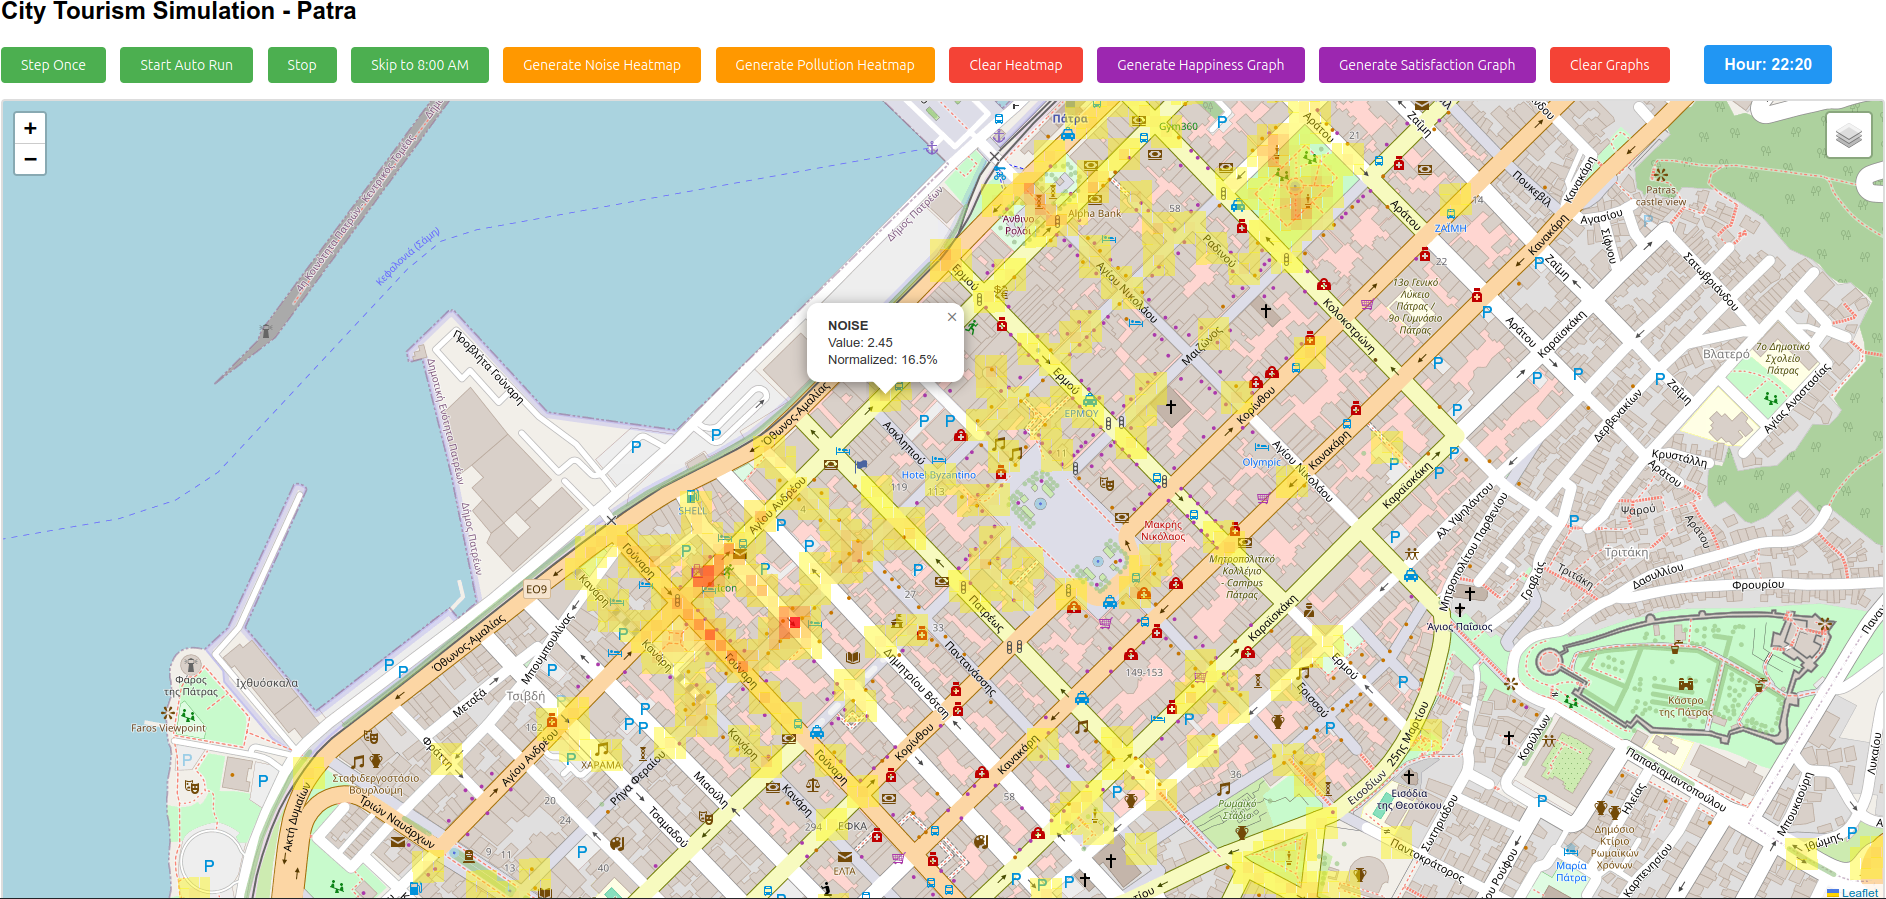
\includegraphics[width=\textwidth]{static/figures/noise_heatmap.png}
\caption{\en{Heatmap} Θορύβου}\label{heatmap}
\end{figure}

\subsection{\en{Charts} Κατανομής Ευτυχίας και Ικανοποίησης}

Τα γραφήματα κατανομών υλοποιούνται με \en{Chart.js} και εμφανίζονται
κάτω από τον χάρτη σε κρυφά \en{div containers} που γίνονται ορατά όταν
ο χρήστης ενεργοποιήσει το αντίστοιχο κουμπί. Κατά την ενεργοποίηση,
καλείται το \en{endpoint /distribution/happiness} ή
\en{/distribution/satisfaction} και τα δεδομένα αποδίδονται ως
ραβδόγραμμα \en{(bar chart)} με 10 \en{bins} στο διάστημα [0.0, 1.0].

Το γράφημα ευτυχίας χρησιμοποιεί μπλε χρωματισμό και εμφανίζει τον
αριθμό κατοίκων ανά εύρος τιμών ευτυχίας, ενώ το γράφημα ικανοποίησης
χρησιμοποιεί μωβ χρωματισμό για τους τουρίστες. Ο συνολικός αριθμός
πρακτόρων κάθε κατηγορίας εμφανίζεται ως τίτλος του γραφήματος. Εάν ο
χρήστης ζητήσει νέο γράφημα, το προηγούμενο καταστρέφεται πριν
δημιουργηθεί το νέο, αποφεύγοντας διπλότυπα \en{instances} του
\en{Chart.js}.

\begin{figure}[H] \centering
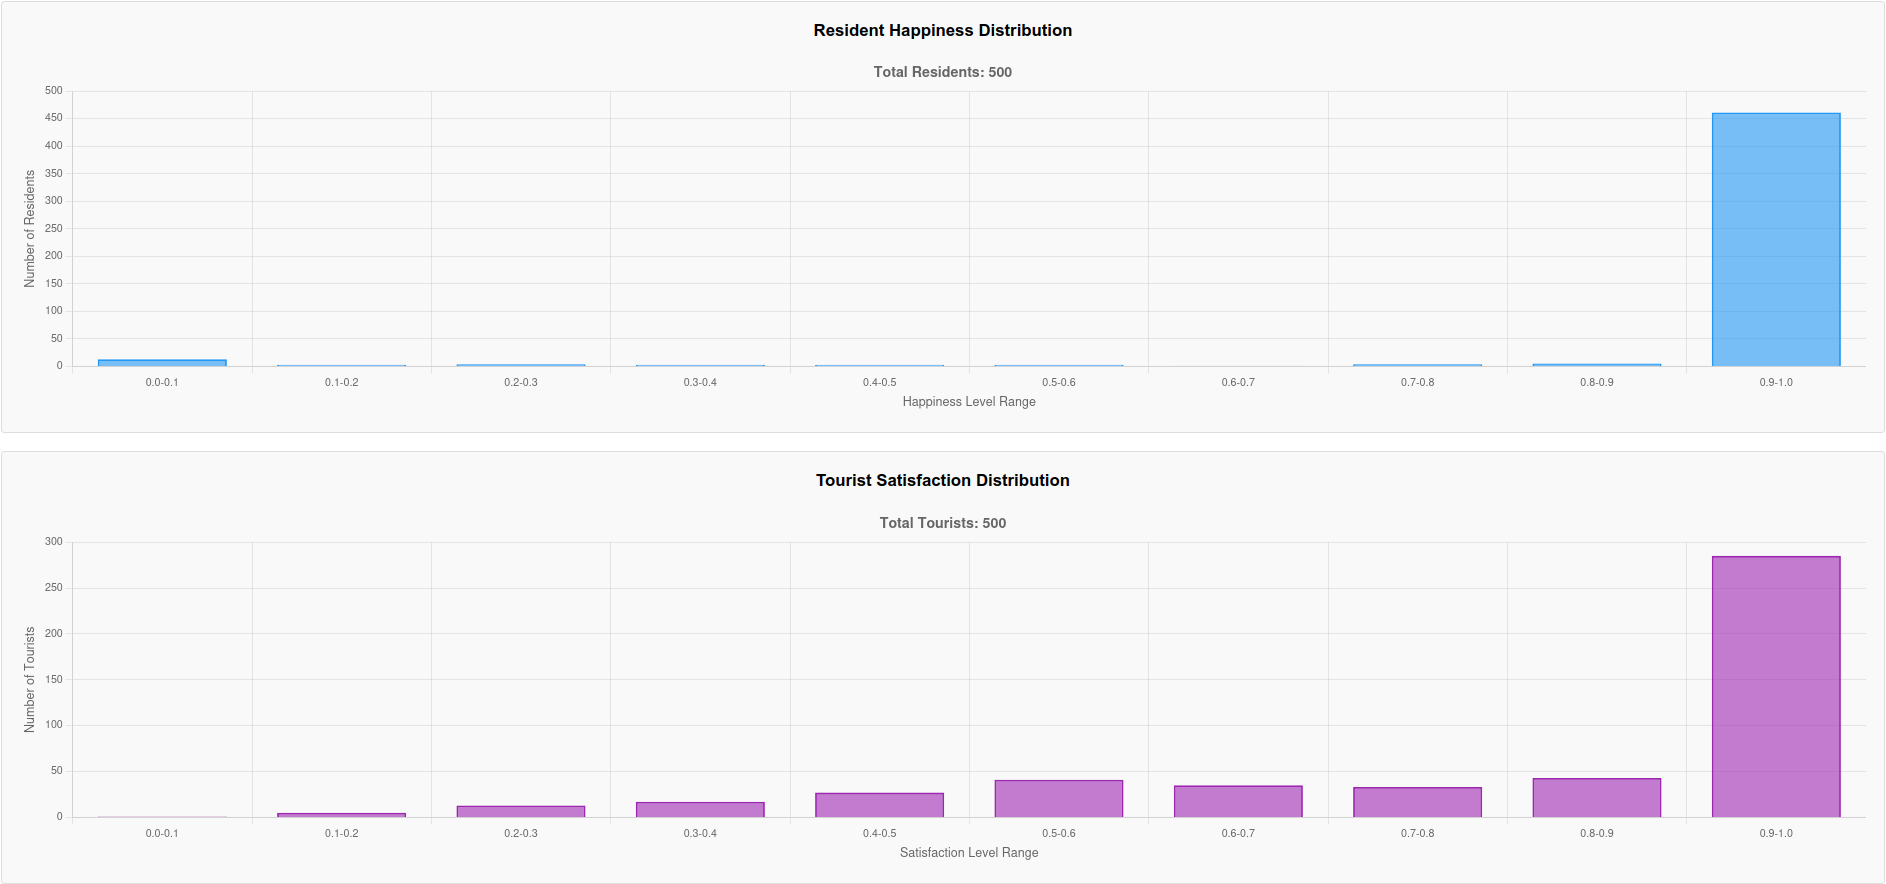
\includegraphics[width=\textwidth]{static/figures/charts.png}
\caption{\en{Charts} Κατανομής Ευτυχίας και Ικανοποίησης}\label{charts}
\end{figure}
	\chapter{Αποτελέσματα και Αξιολόγηση}

Στο κεφάλαιο αυτό παρουσιάζονται τα αποτελέσματα της εκτέλεσης
της προσομοίωσης για τρία σενάρια τουριστικής πίεσης. Αρχικά
ορίζονται τα σενάρια και οι συνθήκες εκτέλεσης, και στη
συνέχεια αναλύονται οι παρατηρήσεις που αφορούν στην
κινητικότητα των τουριστών, στην επίδραση στους κατοίκους,
στην ικανοποίηση των τουριστών και στα \en{heatmaps}
περιβαλλοντικής επίδρασης. Το κεφάλαιο κλείνει με συζήτηση
των περιορισμών του μοντέλου.

\section{Σενάρια Προσομοίωσης}

Η προσομοίωση εκτελέστηκε σε σύστημα με επεξεργαστή
\en{Intel Core i7-9700 @ 3.00GHz}. Λόγω της μονονηματικής
φύσης του \en{Mesa framework}, η εκτέλεση αξιοποιεί έναν μόνο
πυρήνα από τους οκτώ διαθέσιμους. Ως περιοχή μελέτης
χρησιμοποιήθηκε η Πάτρα με \en{buffer} 1.000 μέτρων γύρω από
το κέντρο της πόλης.

Εκτελέστηκαν τρία σενάρια που διαφέρουν ως προς τον αριθμό
τουριστών, με σταθερό αριθμό κατοίκων. Το Σενάριο Α αντιστοιχεί
σε χαμηλή τουριστική πίεση (500 κάτοικοι, 100 τουρίστες),
το Σενάριο Β αντιστοιχεί σε μέτρια τουριστική πίεση
(500 κάτοικοι, 500 τουρίστες), ενώ το Σενάριο Γ σε αυξημένη
τουριστική πίεση (500 κάτοικοι, 1000 τουρίστες). Και στα τρία
σενάρια η προσομοίωση εκτελέστηκε για πλήρες 24ωρο με χρονικό
βήμα 10 λεπτών (144 βήματα συνολικά). Μετρήσεις ελήφθησαν κατά
τη διάρκεια της ημέρας (10:00, 17:00) και στα μεσάνυχτα (23:50),
πριν από την επαναφορά των μεταβλητών.

\section{Παρατηρήσεις επί της Κινητικότητας Τουριστών}

Κατά την εκτέλεση της προσομοίωσης παρατηρήθηκαν χαρακτηριστικά
μοτίβα κινητικότητας που αντικατοπτρίζουν τη λογική του μοντέλου
και, σε μεγάλο βαθμό, τη ρεαλιστική συμπεριφορά τουριστών σε
αστικό περιβάλλον.

Στις 8:00 π.μ., με την έναρξη της ημερήσιας δραστηριότητας, οι
τουρίστες ξεκινούν από τα ξενοδοχεία τους και διασκορπίζονται προς
τα \en{POI Tier A} που εντοπίζουν στην άμεση περιοχή τους. Αυτό
δημιουργεί ένα αρχικό μοτίβο ακτινωτής κίνησης από τα ξενοδοχεία
προς τα αξιοθέατα. Καθώς η ημέρα εξελίσσεται, οι τουρίστες που
έχουν ήδη επισκεφθεί τους πρωτεύοντες στόχους τους μεταβαίνουν
σε κατάσταση \en{casual\_wandering} ή στρέφονται σε
\en{POI Tier B} και \en{C}, με αποτέλεσμα τη σταδιακή διάχυση
της τουριστικής κίνησης στο οδικό δίκτυο.

Ο μηχανισμός \en{forward vision scan} δημιουργεί παρατηρήσιμες
παρεκτροπές, αφού οι τουρίστες που κατευθύνονται προς ένα
\en{Tier A POI} σταματούν σε καφετέριες ή καταστήματα που
εντοπίζουν στο οπτικό τους πεδίο. Αυτό προκαλεί μια φυσική
$``$επιβράδυνση$"$ της κίνησης γύρω από εμπορικούς δρόμους με
υψηλή πυκνότητα \en{Tier B/C POI}, συμπεριφορά που αντιστοιχεί στο
φαινόμενο της παρορμητικής αγοράς που παρατηρείται σε πραγματικούς
τουρίστες. Ιδιαίτερα στα Σενάρια Β και Γ, αυτά τα μοτίβα εντείνονται
και δημιουργούνται εμφανείς ζώνες συγκέντρωσης γύρω από τα
\en{Tier A POI} κατά τις μεσημβρινές ώρες.

\section{Επίδραση Τουρισμού σε Κατοίκους}

Τα αποτελέσματα της κατανομής ευτυχίας κατοίκων αναδεικνύουν με
σαφήνεια την επίδραση της τουριστικής πίεσης στην ποιότητα ζωής.
Οι μόνιμοι κάτοικοι ξεκινούν την μέρα τους με ευτυχία ίση με 0.7,
η οποία μεταβάλλεται ανάλογα με τη πλήθος των τουριστών που έχει
γύρω του ο καθένας.

Στο Σενάριο Α (100 τουρίστες), η ευτυχία των κατοίκων μεταβάλλεται ως
εξής με την πάροδο του χρόνου:

\begin{figure}[H] \centering

\includegraphics[width=\textwidth]{static/figures/500-100/10r.png}
\caption{500 κάτοικοι με 100 τουρίστες (10:00)}\label{figure500-100-10r}
\end{figure}

\begin{figure}[H] \centering

\includegraphics[width=\textwidth]{static/figures/500-100/17r.png}
\caption{500 κάτοικοι με 100 τουρίστες (17:00)}\label{figure500-100-17r}
\end{figure}

\begin{figure}[H] \centering

\includegraphics[width=\textwidth]{static/figures/500-100/23r.png}
\caption{500 κάτοικοι με 100 τουρίστες (23:50)}\label{figure500-100-23r}
\end{figure}

Το Σχήμα~\ref{figure500-100-10r} αναδεικνύει πως μόλις μέσα στις
2 πρώτες πρωινές ώρες, η ευτυχία των περισσότερων κατοίκων ήδη μετέβη
από 0.7 στα μέγιστα επίπεδα. Μόνο ένα μικρό ποσοστό κατοίκων έχει
ευτυχία μικρότερη από 0.9, αλλά κι αυτό σύντομα φτάνει μέγιστα επίπεδα
ευτυχίας σύμφωνα με το Σχήμα~\ref{figure500-100-17r} και το
Σχήμα~\ref{figure500-100-23r}. Αυτή η συμπεριφορά του συστήματος ήταν
αναμενόμενη, λόγω του μικρού πλήθους τουριστών.

Από την άλλη, όταν ο αριθμός των τουριστών πενταπλασιαστεί (500
τουρίστες) τότε τα αποτελέσματα διαφέρουν:

\begin{figure}[H] \centering

\includegraphics[width=\textwidth]{static/figures/500-500/10r.png}
\caption{500 κάτοικοι με 500 τουρίστες (10:00)}\label{figure500-500-10r}
\end{figure}

\begin{figure}[H] \centering

\includegraphics[width=\textwidth]{static/figures/500-500/17r.png}
\caption{500 κάτοικοι με 500 τουρίστες (17:00)}\label{figure500-500-17r}
\end{figure}

\begin{figure}[H] \centering

\includegraphics[width=\textwidth]{static/figures/500-500/23r.png}
\caption{500 κάτοικοι με 500 τουρίστες (23:50)}\label{figure500-500-23r}
\end{figure}

Όπως και στο Σενάριο Α, έτσι και στο Σενάριο Β η πλειοψηφία των κατοίκων
αυξάνει την ευτυχία της στα μέγιστα επίπεδα από τις πρώτες ώρες.
Ωστόσο, ένα μικρό μέρος αυτής της μερίδας κατοίκων μειώνει την ευτυχία της
με τη πάροδο του χρόνου. Εν τέλει, το 5\% των κατοίκων καταλήγει με
μηδενική ευτυχία κατά τα μεσάνυχτα (Σχήμα~\ref{figure500-500-23r}).

Όσον αφορά το Σενάριο Γ,  η κατανομή ευτυχίας των κατοίκων παρουσιάζει
χαρακτήρα παρόμοιο με το Σενάριο Β:

\begin{figure}[H] \centering

\includegraphics[width=\textwidth]{static/figures/500-1000/10r.png}
\caption{500 κάτοικοι με 1000 τουρίστες (10:00)}\label{figure500-1000-10r}
\end{figure}

\begin{figure}[H] \centering

\includegraphics[width=\textwidth]{static/figures/500-1000/17r.png}
\caption{500 κάτοικοι με 1000 τουρίστες (17:00)}\label{figure500-1000-17r}
\end{figure}

\begin{figure}[H] \centering

\includegraphics[width=\textwidth]{static/figures/500-1000/23r.png}
\caption{500 κάτοικοι με 1000 τουρίστες (23:50)}\label{figure500-1000-23r}
\end{figure}

Στις 10:00, η πλειοψηφία των κατοίκων να βρίσκεται στο εύρος 0.9–1.0
(Σχήμα~\ref{figure500-1000-10r}). Καθώς η ημέρα εξελίσσεται, το ποσοστό
κατοίκων που καταλήγει σε μηδενική ευτυχία αυξάνεται στο 8\%
(Σχήμα~\ref{figure500-1000-23r}), έναντι 5\% στο Σενάριο Β. Αυτό επιβεβαιώνει
ότι η επιδείνωση για την πλειονότητα παραμένει οριακή ακόμη και με
διπλασιασμό τουριστών, ενώ η επίδραση εξακολουθεί να συγκεντρώνεται στις
ίδιες ζώνες υψηλής τουριστικής κυκλοφορίας

Το συμπέρασμα είναι ότι ακόμα και στο σενάριο Γ με τους 1000 τουρίστες, η
συντριπτική πλειονότητα των κατοίκων δεν επηρεάζεται σημαντικά. Αυτό
οφείλεται στο γεγονός ότι η τουριστική κίνηση συγκεντρώνεται γεωγραφικά
γύρω από συγκεκριμένα \en{POI} και δρόμους. Οι κάτοικοι που τυχαία
τοποθετήθηκαν σε αυτές τις ζώνες υψηλής πυκνότητας υφίστανται δυσανάλογα
έντονη επίδραση, ενώ οι υπόλοιποι παραμένουν ουσιαστικά ανεπηρέαστοι.

\section{Ικανοποίηση Τουριστών}

Η κατανομή ικανοποίησης των τουριστών παρουσιάζει ενδιαφέρουσα δυναμική
και στα τρία σενάρια. Όλοι οι τουρίστες ξεκινούν την ημέρα τους με 0.7
ικανοποίηση, αλλά αυτή μεταβάλλεται ως εξής κατά τη διάρκεια της ημέρας
στο Σενάριο Α:

\begin{figure}[H] \centering

\includegraphics[width=\textwidth]{static/figures/500-100/10t.png}
\caption{100 τουρίστες (10:00)}\label{figure500-100-10t}
\end{figure}

\begin{figure}[H] \centering

\includegraphics[width=\textwidth]{static/figures/500-100/17t.png}
\caption{100 τουρίστες (17:00)}\label{figure500-100-17t}
\end{figure}

\begin{figure}[H] \centering

\includegraphics[width=\textwidth]{static/figures/500-100/23t.png}
\caption{100 τουρίστες (23:50)}\label{figure500-100-23t}
\end{figure}

Παρατηρείται καθολική άνοδος όσον αφορά την ικανοποίηση των τουριστών,
καθώς ο αριθμός τους δεν είναι επαρκής για να δημιουργήσει συμφόρηση.

Αντίθετα, στο Σενάριο Β ο αριθμός των τουριστών πενταπλασιάστηκε,
γεγονός που μαρτυρούν τα αποτελέσματα:

\begin{figure}[H] \centering

\includegraphics[width=\textwidth]{static/figures/500-500/10t.png}
\caption{500 τουρίστες (10:00)}\label{figure500-500-10t}
\end{figure}

\begin{figure}[H] \centering

\includegraphics[width=\textwidth]{static/figures/500-500/17t.png}
\caption{500 τουρίστες (17:00)}\label{figure500-500-17t}
\end{figure}

\begin{figure}[H] \centering

\includegraphics[width=\textwidth]{static/figures/500-500/23t.png}
\caption{500 τουρίστες (23:50)}\label{figure500-500-23t}
\end{figure}

Κατά τις πρωινές ώρες (Σχήμα~\ref{figure500-500-10t}) η
ικανοποίηση κατά μέσο όρο δεν αποκλίνει πολύ από την αρχική τιμή 0.7.
Όσο περνά ο χρόνος, διαπιστώνεται πως η ικανοποίηση κατανέμεται
σχεδόν ομοιόμορφα για τιμές πάνω από 0.5. Η μεταβλητή παρόλα αυτά
παρουσιάζει σημάδια κλίσης προς τιμές μεγαλύτερες του 0.9
(Σχήμα~\ref{figure500-500-17t}). Όταν φτάσει το πέρας της ημέρας
(Σχήμα~\ref{figure500-500-23t}), η πλειοψηφία συγκεντρώνεται και σε
αυτό το σενάριο σε τιμές μεγαλύτερες του 0.9, αλλά αυτή τη φορά μόνο
το 60\% των τουριστών.

Στο Σενάριο Γ, η εξέλιξη της ικανοποίησης παρουσιάζει το πιο ενδιαφέρον
μοτίβο από τα τρία σενάρια:

\begin{figure}[H] \centering

\includegraphics[width=\textwidth]{static/figures/500-1000/10t.png}
\caption{1000 τουρίστες (10:00)}\label{figure500-1000-10t}
\end{figure}

\begin{figure}[H] \centering

\includegraphics[width=\textwidth]{static/figures/500-1000/17t.png}
\caption{1000 τουρίστες (17:00)}\label{figure500-1000-17t}
\end{figure}

\begin{figure}[H] \centering

\includegraphics[width=\textwidth]{static/figures/500-1000/23t.png}
\caption{1000 τουρίστες (23:50)}\label{figure500-1000-23t}
\end{figure}

Στις 10:00 (Σχήμα~\ref{figure500-1000-10t}) η κατανομή συγκεντρώνεται
γύρω από 0.5–0.6, με σχεδόν κανένα τουρίστα σε ακραίες τιμές.
Στις 17:00 (Σχήμα~\ref{figure500-1000-17t}) η κατανομή $``$πλαταίνει$"$,
κατανεμόμενη σχεδόν ομοιόμορφα σε ολόκληρο το εύρος [0.3, 0.8]. Στα
μεσάνυχτα (Σχήμα~\ref{figure500-1000-23t}) εμφανίζεται χαρακτηριστικά
ένα μεγάλο \en{peak} στο 0.0–0.1 (~130 τουρίστες) και ένα ακόμη
μεγαλύτερο \en{peak} στο 0.9–1.0 (~275 τουρίστες), με  σχετικά
ομοιόμορφη κατανομή στο ενδιάμεσο. Αυτή η πόλωση αντικατοπτρίζει τη
χωρική διαφοροποίηση, όπου τουρίστες που πέρασαν την ημέρα τους σε
κεντρικές ζώνες υψηλής πυκνότητας συσσώρευσαν αρνητικές επιπτώσεις στην
ικανοποίησή τους, ενώ εκείνοι που τυχαία κινήθηκαν σε λιγότερο
πολυσύχναστες περιοχές διατήρησαν ή βελτίωσαν την εμπειρία τους. Το
φαινόμενο αυτό, απόν στα Σενάρια Α και Β, αναδύεται μόνο όταν ο αριθμός
τουριστών φτάσει σε επίπεδο που να δημιουργεί πραγματικό κορεσμό σε
ορισμένα σημεία του δικτύου.

Το τελικό συμπέρασμα είναι πως ακόμα και με μεγάλο πλήθος τουριστών,
η ποιότητα της τουριστικής εμπειρίας παραμένει σε ανεκτά επίπεδα.
Δεν είναι αμελητέο παρόλα αυτά το μέρος των τουριστών που δυσφορεί
από τον συνωστισμό, ειδικά αν προκύψει ακόμα μεγαλύτερη αύξηση
του αριθμού των επισκεπτών.

\section{\en{Heatmaps} Θορύβου και Ρύπανσης}

Τα \en{heatmaps} θορύβου και ρύπανσης αποτυπώνουν χωρικά τη
συγκέντρωση τουριστικής δραστηριότητας στον αστικό χώρο. Οι
υψηλότερες τιμές εμφανίζονται γύρω από τα \en{Tier A POI} και
τους κεντρικούς εμπορικούς δρόμους με υψηλή πυκνότητα
\en{Tier B/C POI}, επιβεβαιώνοντας τη λειτουργία του αλγορίθμου
\en{attractiveness score}.

Η χωρική κατανομή των \en{heatmaps} αναδεικνύει το φαινόμενο της
τουριστικής συγκέντρωσης, όπου ορισμένες ζώνες της πόλης φέρουν
δυσανάλογα υψηλό φορτίο θορύβου και ρύπανσης, ενώ άλλες περιοχές
παραμένουν ουσιαστικά ανεπηρέαστες. Αυτό το μοτίβο είναι
χαρακτηριστικό του υπερτουρισμού και συνδέεται άμεσα με την
παρατηρηθείσα χαμηλή ευτυχία των κατοίκων που τοποθετήθηκαν σε
αυτές τις ζώνες. Στο Σενάριο Γ, οι ζώνες υψηλής συγκέντρωσης
επεκτείνονται και εντείνονται σε σχέση με το Σενάριο Α και Β,
αντικατοπτρίζοντας τις υψηλές ροές των τουριστών.

\begin{figure}[H] \centering
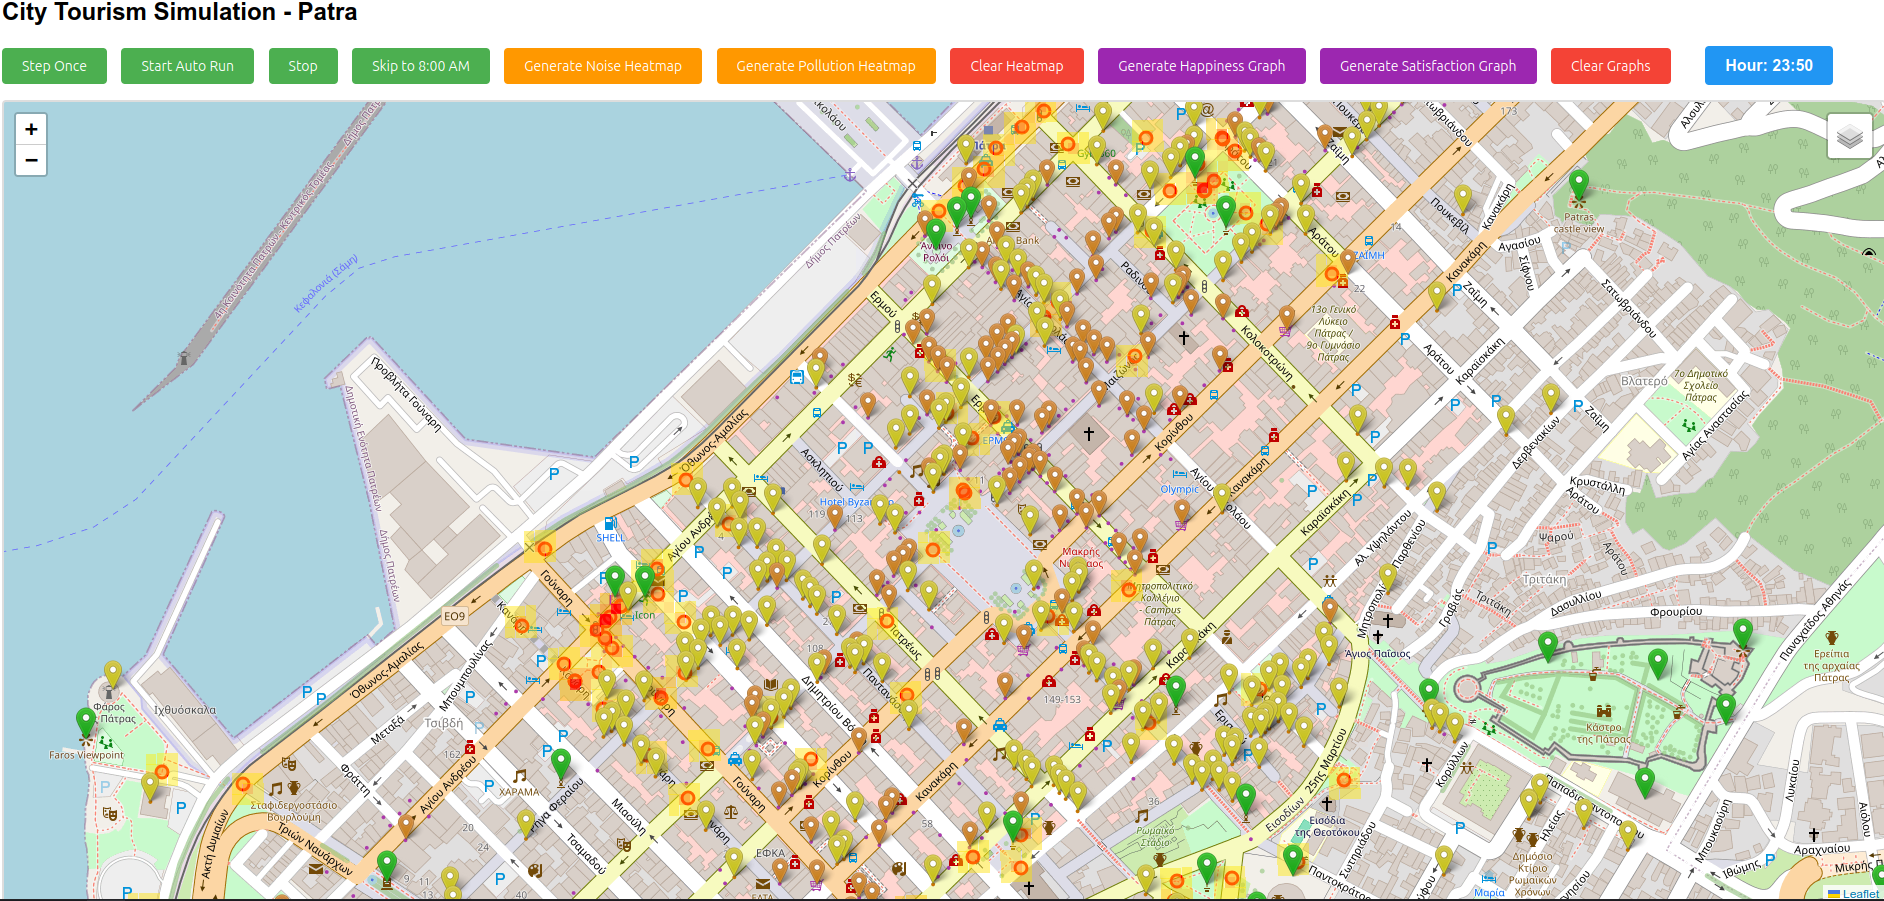
\includegraphics[width=\textwidth]{static/figures/noise_100_23.png}
\caption{100 τουρίστες (23:50)}\label{noise_100_23}
\end{figure}

\begin{figure}[H] \centering
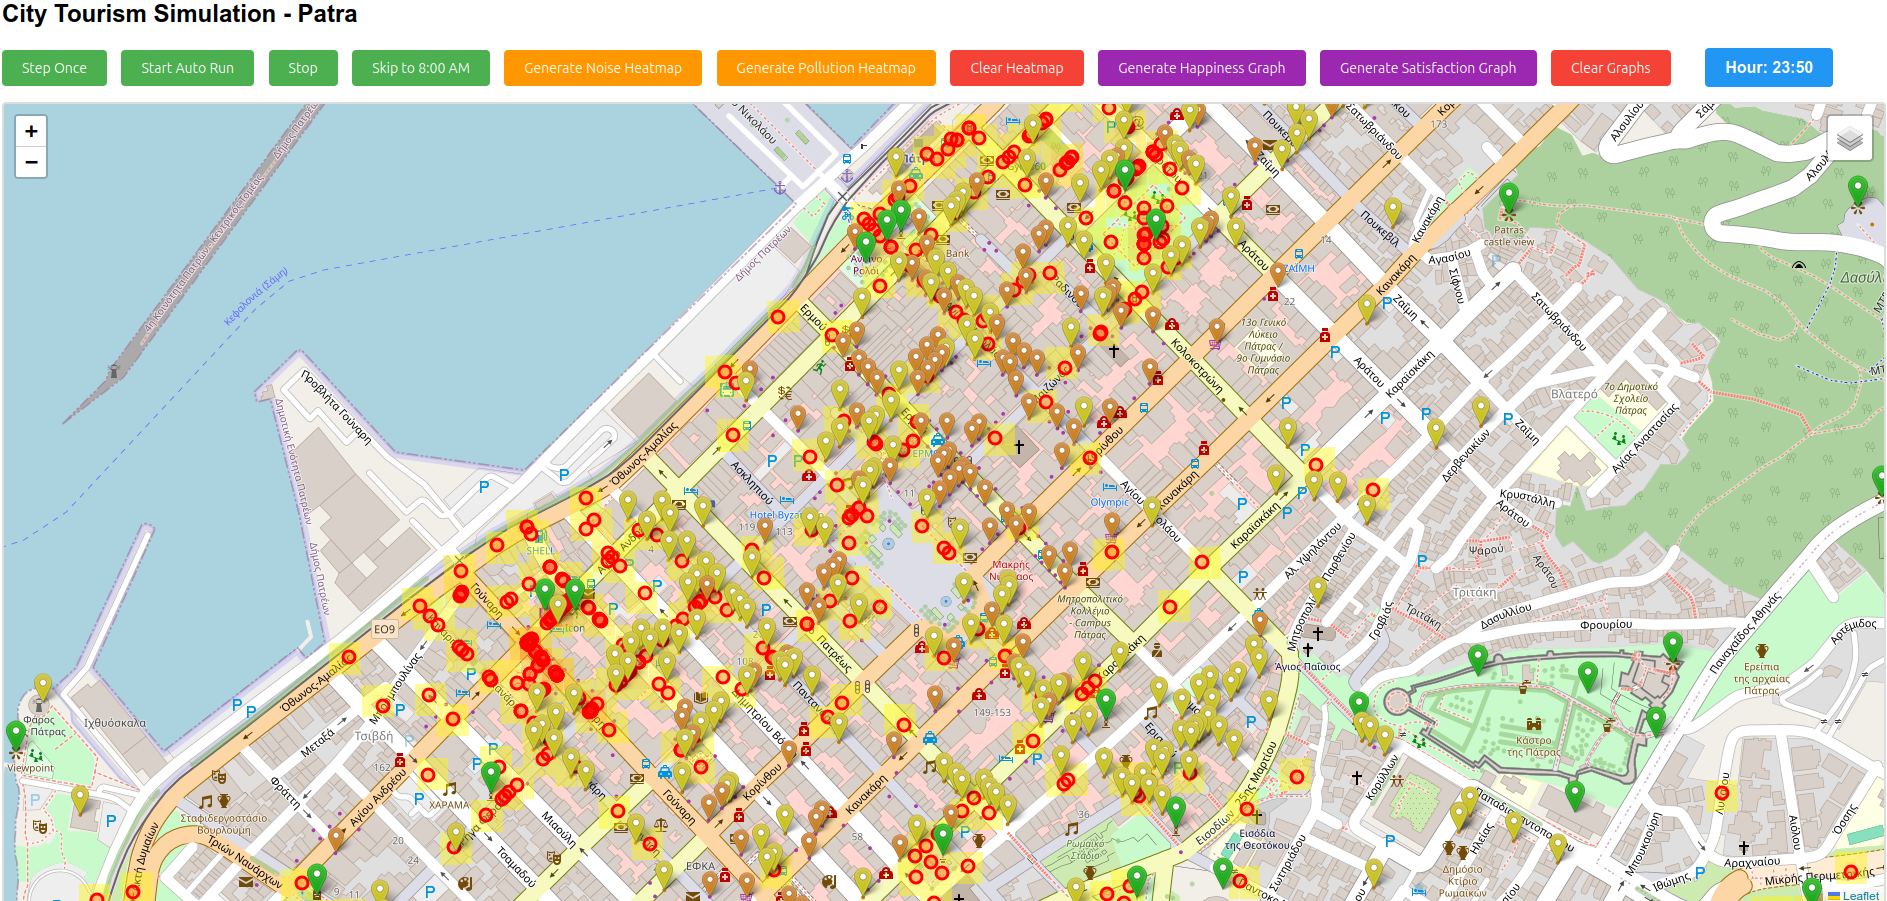
\includegraphics[width=\textwidth]{static/figures/noise_500_23.png}
\caption{500 τουρίστες (23:50)}\label{noise_500_23}
\end{figure}

\begin{figure}[H] \centering
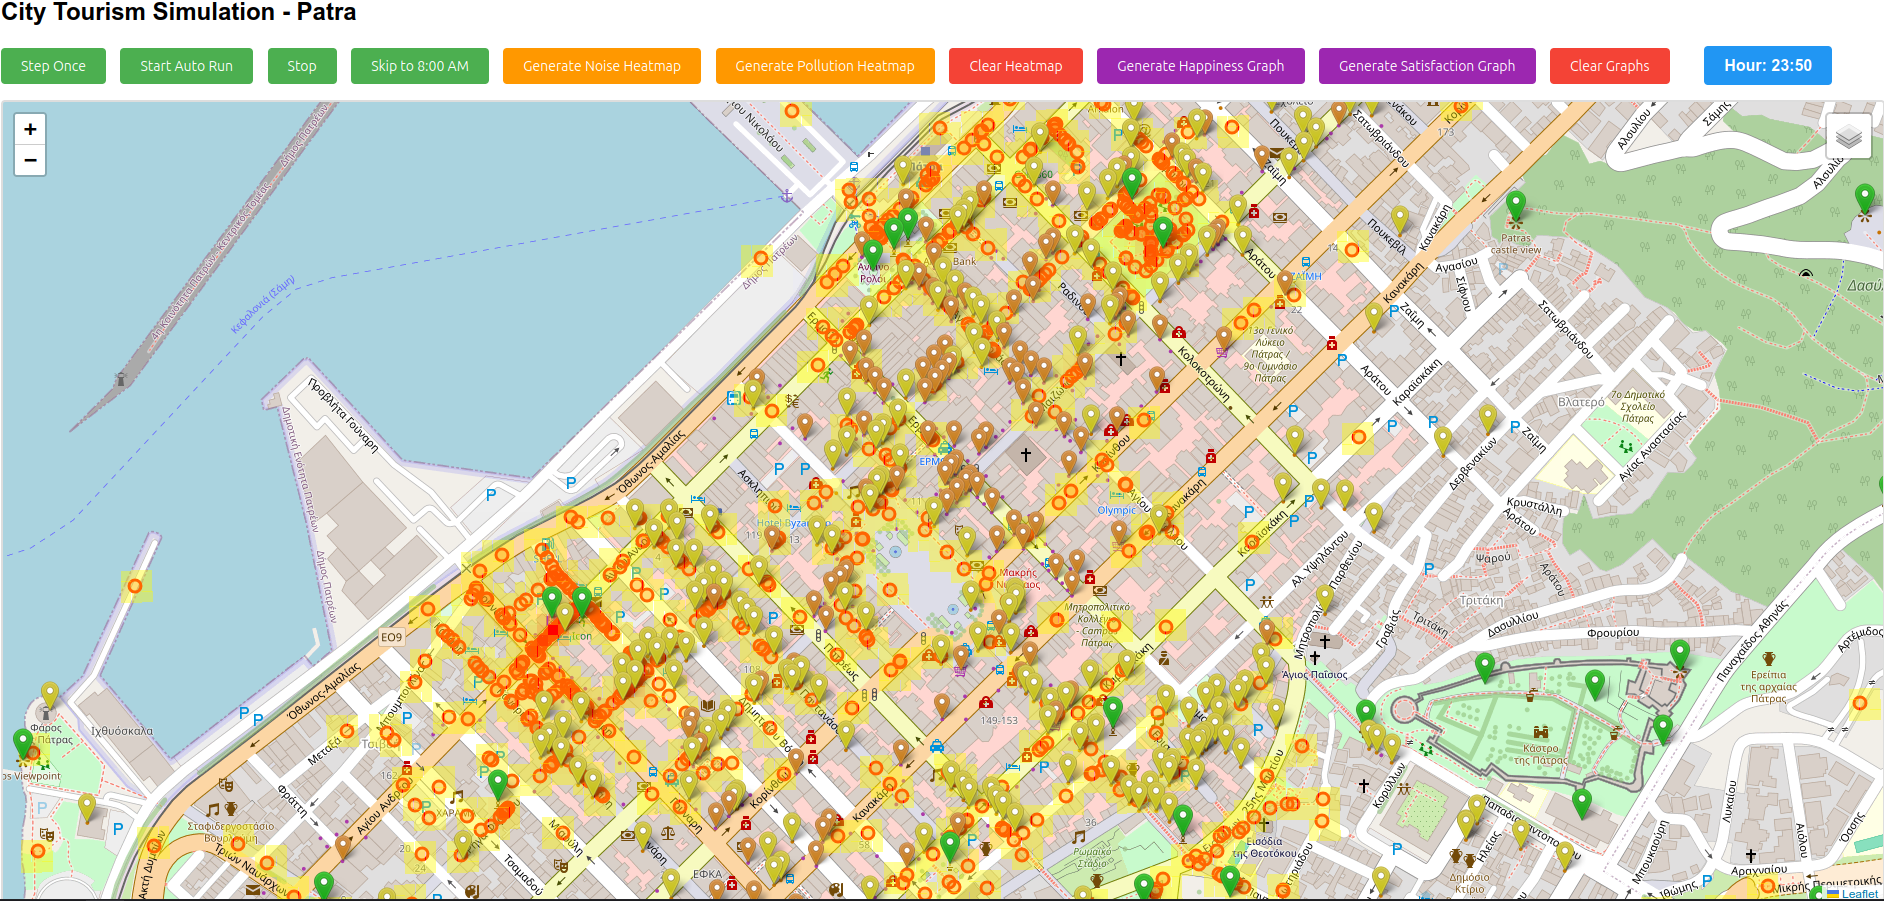
\includegraphics[width=\textwidth]{static/figures/noise_1000_23.png}
\caption{1000 τουρίστες (23:50)}\label{noise_1000_23}
\end{figure}

\section{Περιορισμοί Μοντέλου}

Παρά τα ενδιαφέροντα αποτελέσματα, το μοντέλο παρουσιάζει ορισμένους
περιορισμούς που πρέπει να ληφθούν υπόψη κατά την ερμηνεία των
αποτελεσμάτων.

Πρώτον, οι κάτοικοι είναι στατικοί πράκτορες. Στην πραγματικότητα,
οι κάτοικοι μιας πόλης κινούνται, αλλάζουν περιοχή και προσαρμόζουν
τη συμπεριφορά τους ανάλογα με τον τουρισμό. Η στατικότητά τους στο
παρόν μοντέλο σημαίνει ότι η επίδραση του τουρισμού στην ευτυχία τους
εξαρτάται αποκλειστικά από τυχαία αρχική τοποθέτηση, κάτι που εισάγει
σημαντικό στοιχείο τυχαιότητας στα αποτελέσματα.

Δεύτερον, τα χαρακτηριστικά θορύβου και ρύπανσης κάθε τουρίστα είναι
σταθερά τυχαίες τιμές στο [1, 2], χωρίς διαφοροποίηση βάσει τύπου οδού
ή βάσει κατάστασης (π.χ. διαφορετικές τιμές όταν ο τουρίστας είναι εν κινήσει
και διαφορετικές όταν είναι εντός \en{POI}). Επίσης, η διάχυση στα γειτονικά
κελιά του \en{heatmap} (30\% σταθερό ποσοστό) είναι απλοποιημένη σε σχέση με
ρεαλιστικά μοντέλα ακουστικής ή ατμοσφαιρικής ρύπανσης.

Τρίτον, η προσομοίωση εκτελείται μονονηματικά, γεγονός που περιορίζει την
κλιμάκωση σε μεγάλο αριθμό πρακτόρων. Παρότι ο κώδικας είναι ιδιαίτερα
αποδοτικός—καθώς το \en{Mesa} χρησιμοποιεί χωρική ευρετηρίαση
\en{(spatial indexing)} μέσω εσωτερικού πλέγματος \en{(internal grid)} για
την εύρεση γειτονικών πρακτόρων, ενώ για τον εντοπισμό κοντινών \en{POI}
αξιοποιήθηκε η δομή \en{KD-Tree}—η εκτέλεση περιορίζεται σε μερικές χιλιάδες
πράκτορες λόγω του συνολικού υπολογιστικού κόστους ανά χρονικό βήμα.

Τέλος, τα δεδομένα \en{OSM} για την Πάτρα δεν είναι πλήρη. Ορισμένα
ξενοδοχεία, \en{POI} ή τμήματα οδικού δικτύου ενδέχεται να απουσιάζουν
ή να είναι ανακριβή. Η ποιότητα των αποτελεσμάτων εξαρτάται άμεσα από
την πληρότητα των δεδομένων \en{OpenStreetMap} για την εκάστοτε πόλη.
	\chapter{Επίλογος}

\section{Συμπεράσματα}

Η παρούσα εργασία παρουσίασε ένα σύστημα προσομοίωσης υπερτουρισμού
βασισμένο σε Μοντελοποίηση Πρακτόρων \en{(ABM)}, εφαρμοσμένο στην
πόλη της Πάτρας με χρήση πραγματικών γεωγραφικών δεδομένων 
\en{OpenStreetMap}. Το σύστημα υλοποιεί δύο τύπους πρακτόρων
(μόνιμους κατοίκους και τουρίστες) οι οποίοι αλληλεπιδρούν σε ένα
ρεαλιστικό οδικό δίκτυο, με στόχο την ποσοτικοποίηση της επίδρασης
του τουρισμού τόσο στην ποιότητα ζωής των κατοίκων όσο και στην
εμπειρία των επισκεπτών.

Τα αποτελέσματα των τριών σεναρίων προσομοίωσης αναδεικνύουν τρία βασικά
συμπεράσματα. Πρώτον, η τουριστική πίεση δεν επιδρά ομοιόμορφα στον
χώρο. Ακόμα και με δεκαπλασιασμό των τουριστών, η συντριπτική
πλειονότητα των κατοίκων διατηρεί υψηλή ευτυχία, ενώ η επίδραση
συγκεντρώνεται σε συγκεκριμένες ζώνες υψηλής τουριστικής κυκλοφορίας.
Αυτό το εύρημα υποδεικνύει ότι η χωρική διαχείριση της τουριστικής ροής
(και όχι απαραίτητα η μείωση του συνολικού αριθμού τουριστών)
μπορεί να αποτελέσει αποτελεσματικότερη στρατηγική για τη βελτίωση της
ποιότητας ζωής των κατοίκων.

Δεύτερον, η ικανοποίηση των τουριστών παρουσιάζει αξιοσημείωτη
ανθεκτικότητα. Ακόμα και στο σενάριο υψηλής πίεσης (1000 τουρίστες),
ελάχιστοι είναι οι τουρίστες που παρουσίασαν ικανοποίηση κάτω από 0.2,
ενώ τις βραδινές ώρες το 30\% είχε ανακάμψει σε τιμές 0.9–1.0.
Το εύρημα αυτό υποδηλώνει ότι η χωρική δομή της Πάτρας επιτρέπει
ικανοποιητική διασπορά της τουριστικής κίνησης για τον δοκιμασθέντα
πληθυσμό 1000 τουριστών.

Τρίτον, το σύστημα επιβεβαίωσε την αξία της ιεραρχίας \en{POI} και
του μηχανισμού \en{forward vision scan} ως εργαλείων μοντελοποίησης
ρεαλιστικής τουριστικής συμπεριφοράς. Τα αναδυόμενα μοτίβα κίνησης,
όπως συγκέντρωση γύρω από \en{Tier A POI}, παρεκτροπές σε εμπορικούς
δρόμους και βραδινή αποσυμφόρηση, αντικατοπτρίζουν παρατηρήσεις από
πραγματικά τουριστικά περιβάλλοντα και επιβεβαιώνουν την εγκυρότητα
του μοντέλου.

Συνολικά, η εργασία καταδεικνύει ότι η μοντελοποίηση με πράκτορες
αποτελεί ισχυρό εργαλείο για τη μελέτη υπερτουρισμού, επιτρέποντας
την ποσοτικοποίηση επιπτώσεων που παραδοσιακές μέθοδοι δεν μπορούν
να αποτυπώσουν. Η γεωγραφική γενικευσιμότητα του συστήματος το
καθιστά άμεσα εφαρμόσιμο και σε άλλες ελληνικές πόλεις, παρέχοντας
ένα αναπαραγώγιμο πλαίσιο ανάλυσης.

\section{Μελλοντικές Επεκτάσεις}

Το παρόν σύστημα μπορεί να επεκταθεί σε πολλαπλές κατευθύνσεις. Η
σημαντικότερη βελτίωση θα αφορούσε την ενεργή κίνηση των κατοίκων.
Aντί να είναι στατικοί, οι κάτοικοι θα μπορούσαν να κινούνται στο
οδικό δίκτυο για εργασία, αγορές και αναψυχή, αλλάζοντας δυναμικά
τη γειτνίασή τους ανάλογα με τις τουριστικές ζώνες. Αυτό θα έκανε
τη μεταβλητή ευτυχίας των κατοίκων πολύ πιο ρεαλιστική και λιγότερο
εξαρτημένη από την τυχαία αρχική τοποθέτηση τους.

Μια δεύτερη σημαντική επέκταση είναι η προσθήκη μηχανισμών πολιτικής
διαχείρισης τουρισμού, εμπνευσμένων από τη σχετική βιβλιογραφία.
Για παράδειγμα, θα μπορούσε να υλοποιηθεί σενάριο όπου οι τουρίστες
ενημερώνονται σε πραγματικό χρόνο για τον βαθμό συνωστισμού σε
\en{POI} και αποφεύγουν τα υπερφορτωμένα σημεία, ή σενάριο όπου νέα
\en{Tier A POI} προστίθενται στο μοντέλο για τη διασπορά της
τουριστικής ροής σε μεγαλύτερη έκταση.

Από τεχνική άποψη, η αντικατάσταση του \en{ContinuousSpace} του
\en{Mesa} με χωρικές δομές δεδομένων υψηλής απόδοσης
(π.χ. \en{KDtree} για ερωτήματα γειτόνων εφόσον οι πράκτορες είναι
στατικά σημεία) και η παραλληλοποίηση της εκτέλεσης θα επέτρεπαν την
κλιμάκωση σε χιλιάδες πράκτορες, επιτρέποντας τη μελέτη σεναρίων
μαζικού τουρισμού. Επιπλέον, η βαθμονόμηση του μοντέλου με εμπειρικά
δεδομένα επισκεψιμότητας, εφόσον αυτά είναι διαθέσιμα για την
εκάστοτε πόλη, θα αύξανε σημαντικά την ακρίβεια και την αξιοπιστία
των αποτελεσμάτων.

Τέλος, η ενσωμάτωση χρονικής διακύμανσης της τουριστικής ζήτησης
(εποχικότητα, εβδομαδιαία μοτίβα) και διαφορετικών προφίλ τουριστών
(\en{backpackers}, οικογένειες, ομαδικές εκδρομές) με διαφορετικές
προτιμήσεις \en{POI} και ταχύτητες κίνησης θα προσέδιδε πρόσθετο
ρεαλισμό στο μοντέλο και θα επέτρεπε τη μελέτη πιο εξειδικευμένων
σεναρίων τουριστικής διαχείρισης.

\subsubsection{Σύνδεσμος της εργασίας}
\en{https://github.com/zormpalas/ABM-overtourism}
%	\include{body_matter/chap8}
%	\include{body_matter/chap9}
% Παραρτήματα
	\appendix
%	\include{back_matter/appA}
%	\include{back_matter/appB}	
	\cleardoublepage
% Βιβλιογραφία - Αναφορές
	\bibliography{back_matter/references}
% Συντομογραφίες - Αρκτικόλεξα - Ακρωνύμια
%	\include{back_matter/abbreviations}
% Γλωσσάριο
%	\include{back_matter/glossary}
%%%%%%%%%%%%%%%%%%%%%%%%%%%%%%%%%%%%%%%%%%%%%%%%%%%%
\backmatter
% Ευρετήριο Όρων
	\printindex
	\cleardoublepage

%%%%%%%%%%%%%%%%%%
%%%%%%%%%%%%%%%%%%

%% Δημιουργία ετικετών CD:

%\definecdlabeloffsets{0}{-0.65}{0}{0.55} % upper label x offset [cm] (default=0) /  upper label y offset [cm] (default=0) /  lower label x offset [cm] (default=0) /  lower  label y offset [cm] (default=0) -- For Q-Connect KF01579 labels use the following offset values: {0}{-0.65}{0}{0.55}

%\createcdlabel{Πρότυπο Σύστημα Ομότιμων \\ Κόμβων Βασισμένο σε Σχήματα \en{RDF}}{Κωνσταντίνος Δ. Δημητρίου}{ΟΚΤΩΒΡΙΟΣ}{2014}{8} % τίτλος πτυχιακής / όνομα συγγραφέα / μήνας / έτος / εύρος περιοχής τίτλου σε cm (προτεινόμενη τιμή: 8) 

%%
%% Δημιουργία εξωφύλλου θήκης CD:

%\createcdcover{Πρότυπο Σύστημα Ομότιμων \\ Κόμβων Βασισμένο σε Σχήματα \en{RDF}}{Κωνσταντίνος Δ. Δημητρίου}{ΟΚΤΩΒΡΙΟΣ}{2014}{10} % τίτλος πτυχιακής / όνομα συγγραφέα / μήνας / έτος / εύρος περιοχής τίτλου σε cm (προτεινόμενη τιμή: 10) 

%%
	\pagebreak
	\thispagestyle{empty}
\end{document}